%%%%%%%%%%%%%%%%%%%%%%%%%%%%%%%%%%%%%%%%%%%%%%%%%%%%%%%%%%%%%%%%%%%%%%%%%%%%%%%%%%%%%%%%%%%%%%%%%%%%%%%%%%%%%%%%%%%%%%%%%%%%%%%%%%%%%%%%%%%%%%%%%%%%%%%%%%%
% Manuscript prepared for submission to Frontiers in Bioinformatics (Original Research article)
% using the FrontiersinHarvard.cls template (Frontiers in Bioinformatics uses the Harvard
% author-date reference style; see Frontiers_Journal_style_table.pdf).
%%%%%%%%%%%%%%%%%%%%%%%%%%%%%%%%%%%%%%%%%%%%%%%%%%%%%%%%%%%%%%%%%%%%%%%%%%%%%%%%%%%%%%%%%%%%%%%%%%%%%%%%%%%%%%%%%%%%%%%%%%%%%%%%%%%%%%%%%%%%%%%%%%%%%%%%%%%

\documentclass[utf8]{FrontiersinHarvard}
\usepackage{url,hyperref,lineno,microtype,subcaption}
\usepackage[onehalfspacing]{setspace}
\usepackage{amsmath,amssymb}
\usepackage{textgreek}
% Resolve figures whether they sit in figures/ or at the project root,
% so uploading an image into Overleaf without first opening the figures
% folder still compiles.
\graphicspath{{figures/}{./}}

\linenumbers

\def\keyFont{\fontsize{8}{11}\helveticabold }
\def\firstAuthorLast{Kibler and Dias} % two authors: Frontiers uses "and" (not "et al.") for exactly two
\def\Authors{Ryan Kibler\,$^{1,*}$ and Raquel Dias\,$^{1,*}$}
\def\Address{$^{1}$Department of Microbiology and Cell Science, University of Florida, Gainesville, FL, USA}
\def\corrAuthor{Ryan Kibler}

\def\corrEmail{rkibler@ufl.edu}

\begin{document}
\onecolumn
\firstpage{1}

\title[Co-evolutionary Communities in the EGFR Kinase Domain]{Co-evolutionary Community Architecture of the EGFR Kinase Domain and its Relationship to Conformational Dynamics}

\author[\firstAuthorLast ]{\Authors}
\address{}
\correspondance{}

\extraAuth{Raquel Dias\\ Department of Microbiology and Cell Science, University of Florida, Gainesville, FL, USA\\ raquel.dias@ufl.edu}

\maketitle

\begin{abstract}
\section{}
The Epidermal Growth Factor Receptor (EGFR) is a key oncogenic kinase regulated by long-range allosteric interactions. While most therapeutic strategies target the catalytic site, several clinically important mutations lie outside the immediate catalytic contacts, suggesting that distributed regulatory networks contribute to kinase function. Here, we present a computational framework to map the co-evolutionary architecture of the EGFR kinase domain. Using a redundancy-filtered alignment of 32,912 sequences from the Pfam protein tyrosine and serine/threonine kinase family (PF07714; effective sequence depth $N_{\mathrm{eff}}/L = 109$), we applied Direct Coupling Analysis to infer co-evolutionary constraints and constructed a residue interaction network subject to systematic percolation analysis. This approach identified a critical edge-density threshold at which the network first achieves full connectivity while preserving high modularity ($Q = 0.8036$), partitioning the kinase domain into 15 functional communities. Centrality analysis distinguished structural anchors from inter-module communication bridges, including a dual-role residue at the N-lobe/C-lobe interface and a high-betweenness bottleneck within the hinge region. Inter-module coupling, quantified over the edges defining the partition, was concentrated in a small number of module pairs, with only 63 of 462 edges crossing community boundaries. Five independent 100 ns molecular dynamics simulations of the monomeric domain (500 ns aggregate) showed that the most strongly co-evolving distal residue pairs exhibit a 1.83-fold enrichment in correlated motion relative to a null matched on sequence separation (1.45--1.88 across replicates); however, this enrichment falls to 1.02-fold (bootstrap 95\% CI 0.94--1.12; $p \approx 0.5$) when the null is instead matched on C\textalpha{}--C\textalpha{} distance, and every replicate lies between 0.95 and 1.02 under that control, indicating that the apparent convergence between co-evolution and dynamics in this system is accounted for by three-dimensional proximity rather than by long-range coordination. Against a conformational ensemble of 537 chains from 328 EGFR structures, 43\% of the top-ranked co-evolving pairs prove to be in direct contact in at least one solved state, and no enrichment remains among pairs that stay more than 8~\AA{} apart in every state. Resolving the correlated motion by secondary structure identifies its architectural origin: hydrogen-bonded cross-strand \textbeta{} registers are twice as correlated as other pairs at the same separation, and \textbeta{}-sheet pairs constitute 60\% of the hundred most correlated pairs against a background frequency of 3.8\%, an enrichment that does not extend beyond contact range. Statistical coupling analysis of the same alignment resolves six significant sectors, one of which unites the catalytic lysine K745, the \textalpha{}C-helix glutamate E762, the HRD and DFG motifs and the oncogenic position L858 in a spatially compact network spanning a median sequence separation of 82 residues; its compactness exceeds both conservation-matched and sequence-contiguity-matched nulls, although its membership is itself strongly conservation-correlated. Mapping clinically characterized mutations onto the partition placed the T790M gatekeeper substitution in a hinge-proximal module and the L858R activating substitution in the same community as the DFG aspartate D855, while the minimal coupling route between them follows the backbone and does not constitute a long-range allosteric path. Together, these results provide a community-level description of co-evolutionary organization in the EGFR kinase domain, and delineate which inferences such an analysis can and cannot support.

\tiny
 \keyFont{ \section{Keywords:} EGFR, direct coupling analysis, residue coevolution, allostery, molecular dynamics, community detection, kinase domain, drug resistance}
\end{abstract}

\section{Introduction}

The aberrant cellular signaling that drives oncogenesis is rarely the result of a single residue acting in isolation. Instead, proteins like the epidermal growth factor receptor (EGFR) function as complex molecular circuits, where regulation is distributed across allosteric networks that coordinate conformational changes over long distances \citep{NussinovTsai2013}. Mapping this distributed wiring is critical to understanding how cancer mutations bypass cellular control \citep{Hilser2012}. Traditional structure-based methods have difficulty distinguishing causal communication pathways from background structural correlations \citep{LiuNussinov2016}. Evolutionary sequence analysis offers one complementary window into these networks: when two positions in a protein co-vary across thousands of sequences, it suggests a functional coupling in which mutations at one site are tolerable only when paired with compensating changes at the other \citep{Morcos2011}. Residue interaction network analysis offers a further complementary view by deriving how residues are organized into higher-level community clusters \citep{AstlVerkhivker2019}. When these approaches are combined and cross-validated against protein dynamics, they produce a layered picture of allostery that is more interpretable and more actionable for drug design than any single method yields alone \citep{AstlVerkhivker2019,Sutto2015,Ekambaram2025,Xu2025}.

The kinase domain of EGFR is a well-studied and clinically important instance of distributed regulation in a proto-oncogene. EGFR is a receptor tyrosine kinase whose dysregulation through somatic mutation drives a substantial fraction of non-small cell lung cancers \citep{Zhang2016}. The domain undergoes conformational switching between active and inactive states through coordinated repositioning of the \textalpha{}C-helix, the activation loop, and the catalytic loop \citep{Zhang2006}. Clinically relevant mutations act through more than one mechanism: the T790M resistance mutation substitutes the gatekeeper residue that lines the ATP cleft and confers resistance principally by restoring ATP affinity \citep{Yun2008}, whereas the L858R activating mutation lies in the activation loop and shifts the conformational equilibrium of the domain \citep{Behn2025}. Structural studies have further established that EGFR activation is itself an allosteric event, in which the C-terminal lobe of one kinase molecule stabilizes the active conformation of a second through the \textalpha{}G-helix region \citep{Zhang2006,Jura2009}. Prior computational work has characterized allosteric communication pathways in EGFR using simulation-based network models \citep{DixitVerkhivker2011}, yet these approaches do not incorporate the evolutionary record of sequence variation across the protein family. Halabi and colleagues \citep{Halabi2009} established that kinase domains are organized into co-evolving residue communities, termed sectors, which represent approximately independent evolutionary units linked to distinct functional aspects. \citet{Sutto2015} subsequently demonstrated that statistical couplings within such alignments can predict the physical dynamic behavior of kinase family members.

While the broad evolutionary principles of the protein kinase superfamily have been extensively mapped \citep{Halabi2009,Sutto2015}, the community-level organization of those constraints within the EGFR kinase domain has not been described at a principled network resolution. Because PF07714 spans tyrosine and serine/threonine kinases across eukaryotes, the couplings recovered here reflect constraints conserved across the kinase superfamily rather than features specific to receptor tyrosine kinases or to the ErbB family; resolving ErbB-specific architecture would require a subfamily-restricted alignment, a limitation we return to in Section~\ref{sec:limitations}. Although AlphaFold2 has transformed static structure prediction \citep{Jumper2021}, it generates single ranked structures that do not capture the conformational ensembles underlying allostery \citep{Nussinov2022,Bowman2024}, leaving the dynamic residue networks governing EGFR signaling undercharacterized. Comparing evolutionary clusters against conformational dynamics allows us to assess whether statistical co-evolutionary hubs correspond to structural elements of the kinase domain, and\textemdash critically\textemdash whether any apparent correspondence survives control for three-dimensional proximity \citep{Sutto2015}.

We hypothesize that the EGFR kinase domain is organized into a modular co-evolutionary architecture whose high-centrality residues correspond to identifiable structural elements, and we ask whether these evolutionary constraints are reflected in correlated conformational fluctuations beyond what spatial proximity alone predicts. To assess this, we implemented large-scale sequence alignment, pairwise co-evolutionary scoring via pseudolikelihood maximization, and graph-theoretic community detection, combined with molecular dynamics simulation and statistical validation.

\section{Results and Discussion}

\subsection{A Deeply Sampled, Redundancy-Filtered Kinase Alignment Provides a Foundation for Co-evolutionary Analysis}

In order to characterize evolutionary variation across the kinase family to which the EGFR catalytic domain belongs, we used the full alignment of Pfam family PF07714 and processed it through the filtering pipeline described in Methods. PF07714 is designated \emph{Protein tyrosine and serine/threonine kinase} (previous identifier \emph{Pkinase\_Tyr}) and therefore spans both tyrosine and serine/threonine kinase catalytic domains.

We found that after filtering, the alignment retained 32,912 sequences, each spanning 3,839 alignment columns, with the human EGFR reference sequence confirmed present. EGFR\_HUMAN/712-968 occupies 257 alignment positions, of which 253 are match-state columns; these 253 positions, corresponding to residues 714 through 966, constitute the focus set carried into the coupling analysis (Figure~\ref{fig:overview}B).

The initial data set contained 400,321 sequences, with heavily sequenced lineages overrepresented, hence any co-variation signal calculated from the raw alignment would be dominated by shared ancestry rather than genuine functional constraint. To correct for this, sequences were clustered at 62\% identity, which removed redundant entries while preserving the phylogenetic breadth of the family. The retained alignment has an effective sequence depth of $N_{\mathrm{eff}} = 27{,}613$ after similarity reweighting, i.e. $N_{\mathrm{eff}}/L = 109$ for $L = 253$ scored positions, which is well above the depth at which direct coupling analysis scores are considered reliable \citep{Ekeberg2013}.

We note two consequences of this filtering that bear on interpretation. First, because the alignment was reduced to 62\%-identity cluster representatives before reweighting, the subsequent 80\% downweighting threshold had almost no effect: the mean 80\%-identity neighbourhood of the retained sequences is 1.000. Second, aggressive clustering preferentially discards mutually similar sequences, and the retained set is correspondingly depleted of close EGFR relatives: vertebrate sequences fall from 35.8\% of the raw family to 3.5\% of the retained alignment, which contains two human sequences and a single ErbB-family sequence, namely the manually recovered EGFR reference itself. The couplings reported below therefore describe constraints conserved across the kinase superfamily rather than ErbB-specific or receptor-tyrosine-kinase-specific features. The human EGFR sequence (EGFR\_HUMAN/712-968) was not selected as a cluster representative at the 62\% cutoff, so it was retrieved separately from the original alignment and appended to the filtered set, ensuring that all downstream residue numbering maps correctly to the human protein. The 257 alignment columns occupied by the EGFR\_HUMAN sequence were identified and recorded, so that coupling scores could subsequently be reported in human EGFR residue numbers rather than alignment column indices.

This alignment represents a resource of considerably greater depth and phylogenetic diversity than those used in prior structure-based network analyses of the ErbB family \citep{JamesVerkhivker2014}, although, as noted above, that diversity is achieved at the cost of subfamily-specific signal.

\subsection{Pseudolikelihood Co-evolutionary Scoring Recovers 31,878 Residue Pair Constraints Across the EGFR Kinase Domain}

To determine which pairs of positions in the EGFR kinase domain are subject to coupled evolutionary pressure, we applied a pseudolikelihood-based pairwise co-evolutionary scoring method to the filtered alignment, focused on the 253 match-state EGFR positions, as described in Methods.

We found that the analysis produced coupling scores for all 31,878 unique residue pairs within the EGFR focus region, equal to the $\binom{253}{2}$ pairs formed by the 253 scored positions. Scores summarize the strength of direct statistical co-variation between each pair after indirect correlations have been removed, and are average-product-corrected; they are therefore signed, with a mean of approximately zero across all pairs (mean 0.0004; range $-1.78$ to $6.38$; 55.5\% negative). Positive values indicate coupling above the phylogenetic and entropic background, and this sign convention is important for the inter-module analysis in Section~\ref{sec:flux}.

The key distinction between the method utilized and simpler alternatives is handling of indirect correlations. If position A co-varies with position B, and position B co-varies with position C, a naive correlation measure will report a signal between A and C even if they have no direct functional relationship. The pseudolikelihood approach fits a global statistical model to the entire alignment simultaneously, which allows it to distinguish pairs that co-vary because they genuinely constrain each other from pairs that appear coupled only because both happen to co-vary with a third position \citep{Ekeberg2013,Halabi2009}. Phylogenetic weighting was applied so that groups of sequences with more than 80\% identity between them collectively counted as a single observation rather than inflating the apparent sample size, and regularization was used to prevent the fitting procedure from over-explaining the data. The calculation was run for 500 iterations to ensure a resolution appropriate for detecting subtle allosteric constraints, requiring 8 CPU cores, 64 GB of RAM, and approximately 24 hours on a shared computing cluster. Each pair's score is a single number summarizing the full matrix of coupling parameters between the two positions, giving a scalar value that can be ranked and thresholded for network construction.

The breadth of the scored pairs spanning the full 253-position focus set, rather than clustering exclusively near the ATP pocket, is consistent with the idea that evolutionary constraints in this family reflect distributed regulation rather than a localized catalytic constraint, which supports the framing of this analysis as a search for allosteric modules \citep{AstlVerkhivker2019,Sutto2015}.

\subsection{Topological Foundation: Percolation Analysis}

To convert the 31,878 pairwise coupling scores into a tractable network representation of the EGFR co-evolutionary architecture, a threshold was required to define which couplings represent meaningful evolutionary constraints. Rather than selecting this cutoff arbitrarily, we performed a systematic topological percolation analysis in which networks were constructed at edge densities ranging from $1.0L$ to $4.0L$ ($L = 253$ scored positions) in increments of $0.05L$. For each network, we recorded the fraction of the 253 analyzable focus residues contained in the largest connected component (LCC) and the modularity score ($Q$) of the Louvain partition (Figure~\ref{fig:percolation}).

We observe a clear trade-off between connectivity and modular resolution across this density range. At the lowest threshold tested ($1.0L$; 253 edges), the Louvain algorithm yielded the highest modularity value ($Q = 0.8894$, 21 communities); however, this network incorporated only 50.2\% of the analyzable focus residues into a connected component and therefore cannot serve as a representation of domain-wide co-evolutionary communication. Modularity decreases monotonically from this point as edges are added, so the threshold adopted below is not a modularity optimum. As the threshold increased, connectivity improved until, at 458 edges, all 253 analyzable residues were first incorporated into a single connected component; at 457 edges the largest component contains 252 of 253 residues. All downstream analyses use the 462-edge network ($Q = 0.8036$ under weighted Louvain), four edges above this transition. This edge density corresponds to the critical percolation point, defined as the minimum density at which a single giant component spanning the full analyzable domain first emerges. Networks constructed below this threshold are necessarily fragmented and preclude inference of global inter-module pathways; networks above it accumulate progressively weaker edges that erode modular structure without improving connectivity.

To assess the robustness of downstream conclusions to this choice, we re-ran the analysis across a $\pm$10\% variation in threshold density (404 to 506 edges). Robustness is not uniform across quantities. The highest-strength residues are stable: 965, 717, 799, 851 and 964 occupy the top five positions by node strength at every threshold tested. The number of detected communities is not stable, varying between 14 and 16 over the same window, and the betweenness ranking is also threshold-dependent: at 404 and 430 edges the highest-betweenness residue is 849, which does not appear among the top five at 462 edges. Conclusions resting on node strength are therefore better supported than those resting on community count or betweenness rank, and we qualify the corresponding statements below accordingly.

Community detection performed on the $1.80L$ network using the Louvain algorithm (resolution parameter $\gamma = 1.0$) across 100 independent random initializations partitioned the 253 analyzable residues into 15 communities. Community sizes ranged from large structural scaffolds, such as Community 3 (C-lobe Core/Tail Base; 32 residues), to compact regulatory modules such as Community 11 (7 residues). The spatial coherence of these communities, assessed by mapping onto the erlotinib-bound EGFR kinase domain structure (PDB: 1M17) \citep{Stamos2002} and a full-length AlphaFold2 model (UniProt: P00533) \citep{Jumper2021,UniProt2023}, confirmed that all 15 communities correspond to physically contiguous three-dimensional regions, consistent with the interpretation that the evolutionary modules reflect structurally localized functional units. Having established this community partition at a principled, validated threshold, we next characterized the influence of individual residues within the resulting network.

\subsection{Infrastructure vs. Communication: Centrality Analysis}

Within the $1.80L$ network, we distinguished two complementary classes of influential residues using distinct centrality metrics. Node strength, defined as the sum of raw coupling weights ($J_{ij}$) incident to each node, identifies residues that serve as high-connectivity structural anchors within their local module. Betweenness centrality, defined as the fraction of all-pairs shortest paths (computed using path lengths defined as $1/J_{ij}$) passing through a given node, identifies residues that serve as information bridges between modules. These two metrics capture fundamentally different aspects of network influence and are reported separately to avoid conflating local integration with global communication (Figure~\ref{fig:centrality}).

By node strength, the five strongest hubs were residues 965 (24.74), 717, 799, 851, and 964. Residue 965, the highest-strength node in the network, warrants a structural caveat: this site lies within the C-terminal tail, a region frequently disordered and unresolved in crystallographic models including PDB 1M17. Its high node strength therefore reflects strong sequence-derived co-evolutionary constraints inferred from the multiple sequence alignment rather than observed structural contacts in static models. Its placement at high centrality is nevertheless consistent with the AlphaFold2 model, in which residue 965 is positioned at the interface between the disordered tail and the folded catalytic core. Residues 883 and 884 lie within the \textalpha{}F-helix, the structural anchor of the regulatory spine, but do not rank among the primary infrastructure hubs of this network: they place 112th and 98th of 253 by node strength respectively. A network knockout analysis is consistent with this: removing residue 793 reduces global network efficiency by 2.26\%, and removing 858 or 965 by 1.44\% and 1.00\%, whereas removing 884 or 733 changes it by less than 0.03\% in the opposite direction. We therefore do not claim a hub role for the \textalpha{}F-helix residues on the basis of this network.

By betweenness centrality, the five primary inter-module bridges were residues 792 (normalized betweenness: 0.311), 838, 793 (0.265), 853, and 852. The concentrated betweenness at residues 792 and 793 identifies the hinge region as the principal bottleneck for information flow between the N- and C-terminal lobes of the kinase domain in this network, subject to the threshold sensitivity of betweenness noted above. Residue 793 represents an exceptional dual-role node, ranking within the top 10 by both node strength (18.32) and betweenness centrality (0.265), a combination that suggests this position simultaneously stabilizes a local structural module and mediates cross-module communication. The dual-role character of residue 793 and the bottleneck architecture at the hinge region carry direct implications for drug resistance mechanisms, which are addressed in Section~\ref{sec:mutationmapping}.

We note that centrality metrics depend on network construction and weighting schemes; therefore, these values should be interpreted as relative indicators of topological influence rather than direct measures of functional importance.

To determine whether these topological features are reflected in the physical behavior of the domain, we next analyzed the conformational dynamics of each community using molecular dynamics simulation.

\subsection{Mechanical Partitioning: RMSF Analysis}

To assess whether the evolutionary community partition corresponds to a physically meaningful segmentation of the kinase domain's conformational dynamics, we performed five independent 100 ns molecular dynamics simulations of the EGFR kinase domain (residues 712-970), 500 ns in aggregate, using GROMACS 2025.2 \citep{Abraham2015} with the AMBER99SB-ILDN force field \citep{LindorffLarsen2010} and explicit TIP3P solvent \citep{Jorgensen1983} at 310 K and 1 bar. Conformational flexibility was quantified using per-residue root-mean-square fluctuation (RMSF) calculated from each production trajectory, and mean RMSF values were aggregated at the community level (Figure~\ref{fig:rmsf}). Values quoted below are from replicate 1, the trajectory on which the remaining analyses were computed; their reproducibility across replicates is reported in Section 2.9.

We observe a clear mechanical hierarchy across the 15 communities. The Regulatory \textalpha{}C-Helix (Community 7) exhibited the highest mean fluctuation (0.2135 nm), consistent with its established role as the primary conformational switch during kinase activation. The \textbeta{}1--\textbeta{}3 N-lobe framework (Community 0; mean RMSF = 0.1721 nm) and the P-loop/N-lobe core (Community 1; 0.1715 nm) communities also showed substantial flexibility, consistent with their involvement in nucleotide binding and positioning. In contrast, the catalytic loop/\textalpha{}F module (Community 14; 0.0636 nm) and the C-lobe core (Community 3; 0.0545 nm) were the most rigid regions, functioning as the structural scaffold supporting catalytic geometry. The resulting 3.9-fold gradient between the most dynamic community (Community 7) and the most rigid (Community 3) provides a community-level mechanical partition of the kinase domain; the corresponding ratio against the catalytic loop/\textalpha{}F module (Community 14) is 3.4-fold. The ordering is reproducible: Community 7 is the most mobile and Community 3 the most rigid module in all five replicates. The magnitude of the gradient is more variable, spanning 2.8--4.0-fold for Community 7 over Community 3 and 1.9--3.4-fold over Community 14 across replicates, with replicate 1 at the upper end of both ranges (Section 2.9).

We note that these results represent the intrinsic vibrational modes of a single 100 ns conformational ensemble of the monomeric domain, initiated from the active-state crystal structure, and that the simulated construct terminates at residue 970. Residue 965 therefore lies five residues from a free chain end and the C-terminal tail (971--1210) is absent entirely, so dynamic quantities reported at the extreme C-terminus of the construct are not interpretable as tail behaviour. The directionality of the observed gradient is physically interpretable, consistent with established structural knowledge of kinase mechanics, and reproduced in every replicate; the absolute RMSF values are the replicate-dependent quantity, and we accordingly interpret the ordering of the communities rather than the magnitude of their fluctuations (Section 2.9). These dynamics provide a representative foundation for the cross-correlation analysis that follows.

\subsection{Inter-Module Coupling}
\label{sec:flux}

Having established the modular partition and its mechanical character, we next asked how co-evolutionary coupling is distributed between communities. For each pair of communities ($A$, $B$) the cumulative coupling $\Phi_{AB} = \sum_{i \in A, j \in B} J_{ij}$ can be computed over all $|A| \times |B|$ residue pairs (Figure~\ref{fig:flux}). Because the coupling scores are average-product-corrected and therefore signed with a mean of approximately zero (Section 2.2), this sum is dominated by background accumulation rather than by coupling strength: 75 of the 105 community pairs return a negative value, and $\Phi$ is negatively correlated with the number of contributing pairs ($r = -0.33$, $p = 5.5 \times 10^{-4}$). A negative cumulative value cannot be interpreted as evolutionary pressure maintaining coordination, and we therefore do not use this quantity to rank pathways.

Instead we report inter-module coupling restricted to the 462 edges that define the network partition, which is both well posed and internally consistent with how the communities were obtained. Under this measure, inter-module coupling is sparse and concentrated: only 63 of the 462 edges cross community boundaries, distributed across 27 of the 105 possible module pairs, as expected for a partition of high modularity ($Q = 0.8036$). The strongest inter-module channels connect Community 3 to Community 6 (8 edges, $\sum J_{ij} = 18.01$) and Community 3 to Community 14 (7 edges, $\sum J_{ij} = 12.95$), both within the C-lobe scaffold. Ranking by coupling density, $\Phi_{AB}/(|A| \times |B|)$, as defined in Methods, gives a third ordering again, led by the Community 2--Community 4 pair. Because these three well-defined statistics do not agree, we refrain from designating any module pair as a dominant allosteric conduit.

Two specific observations warrant comment, because both were prominent in an earlier version of this analysis that ranked module pairs by the signed cumulative sum. First, the Community 1--Community 7 pair, which joins the P-loop/N-lobe module to the regulatory \textalpha{}C-helix module, is connected by a single edge in the 462-edge network and ranks 22nd of 105 by inter-module coupling over those edges. Recovery of this pair therefore cannot be presented as a positive methodological validation of the approach. Second, the pair joining Community 5 (residues 909--922, the \textalpha{}G--\textalpha{}H loop) to Community 10 (residue 908 together with residues 923--943, spanning the \textalpha{}H region) is connected by three edges, of which two, 922--923 and 908--909, are immediately sequence-adjacent backbone pairs and the third, 918--926, spans eight residues. Community 10 flanks Community 5 on both sides in sequence. This channel therefore reflects backbone continuity between consecutive C-lobe segments rather than long-range coupling, and the $|i-j|>5$ filter applied to the dynamic analyses in Section 2.8 would have removed it. We note additionally that the canonical activator-side residues of the asymmetric kinase dimer, V948, M952 and I953 in UniProt P00533 numbering, fall in Communities 3, 11 and 11 respectively and in neither Community 5 nor Community 10, and that V948 ranks 182nd of 253 by node strength. We accordingly do not interpret this channel as a conduit linking the dimerization interface to the C-terminal tail anchor.

\subsection{Convergence of Evolution and Dynamics: DCA vs. DCCM}

To determine whether the evolutionary co-variation encoded by Direct Coupling Analysis (DCA) is reflected in the physical coordination of residue motion captured by molecular dynamics, we computed a Dynamic Cross-Correlation Matrix (DCCM) from the production trajectory and examined the correspondence between the two representations (Figure~\ref{fig:dccm}).

The DCCM revealed a localized region of strong positive correlation spanning residues 760-853, visible as a discrete cluster in the heatmap. This region encompasses the \textalpha{}C-helix and the DFG motif of the activation loop, two structural elements that move in concert during kinase activation. We note that correlated motion within a contiguous structural region is expected on mechanical grounds, and Section 2.8 assesses whether any such correspondence exceeds what spatial proximity alone predicts.

To identify pairs exhibiting a strong simultaneous signal in both representations, we computed a consensus score defined as the product of the DCA coupling weight and the absolute DCCM correlation coefficient for each distal pair. This ranking proves sensitive to the sequence-separation filter applied, and we report it with that caveat. Under the $|i-j|>5$ filter used elsewhere in this work, the maximum is residue pair 717-725 (consensus score 3.66), 49\% ahead of the runner-up. Under a more restrictive $|i-j|>10$ filter the maximum is instead residue pair 799-841 (consensus score 2.33, sequence separation 42), which links the \textalpha{}D-helix core to the catalytic loop, but its margin over the runner-up (728-741, 2.31) is 0.7\%. A preprint version of this work reported 799-841 as the global maximum of this distribution; that statement holds only under the more restrictive filter and by a margin smaller than any reasonable estimate of the uncertainty in a single-trajectory DCCM. We therefore do not designate any single pair as the locus of evolutionary--dynamic convergence, and note that the analysis in Section 2.8 supersedes this ranking in any case.

Residue 965 showed a mean absolute DCCM correlation with the catalytic core of 0.161, against a random distal baseline of 0.156. This 3\% difference derives from a trajectory in which residue 965 lies five residues from a truncated chain terminus, and it is far smaller than the variation in the overall level of dynamic correlation between independent trajectories, which spans 0.280--0.422 for the co-evolving set across the five replicates (Section 2.9); we regard it as indistinguishable from noise rather than as evidence of tail-mediated communication.

\subsection{Statistical Integration and Significance}

To quantify the relationship between evolutionary co-variation and dynamic correlation, we compared the absolute DCCM values of the 500 residue pairs connected by the highest-ranking co-evolutionary couplings against two null distributions, each of 500 randomly selected pairs.

Against a null matched only on sequence separation ($|i-j|>5$, the filter used throughout), co-evolving distal pairs exhibited a mean absolute dynamic correlation of 0.287 compared with a baseline of 0.157, a 1.83-fold enrichment, with a nominal two-sample $t$-test $p$-value of $1.1 \times 10^{-33}$. This reproduces the enrichment reported in the preprint version of this analysis, and the enrichment is recovered in all five replicates (1.45--1.88; Section 2.9).

This comparison does not, however, control for the variable that governs dynamic correlation most strongly. Direct coupling analysis preferentially recovers residue pairs that are in spatial contact \citep{Morcos2011}, and residues in contact move together for mechanical reasons independent of any allosteric mechanism. The top 500 co-evolving pairs have a median C\textalpha{}--C\textalpha{} separation of 11.4~\AA{} against 24.3~\AA{} for the remaining distal pairs, so a sequence-separation filter leaves this confound intact. We therefore constructed a second null matched on C\textalpha{}--C\textalpha{} distance in 2~\AA{} bins. Against this distance-matched null the mean absolute correlation of the co-evolving set is 0.287 versus 0.281, an enrichment of 1.02-fold (bootstrap 95\% CI 0.94--1.12; $p \approx 0.5$, two-sample $t$-test; Mann--Whitney $p \approx 0.6$). The ratio is stable across resampling seeds; the $p$-value is quoted to one decimal because the draw-to-draw spread makes further digits unstable, and the confidence interval is the inferential statement. It is also stable across independent trajectories: per-replicate enrichment under this null spans 0.95--1.02 and every per-replicate bootstrap interval includes unity (Section 2.9). Consistently, the partial rank correlation between coupling strength and absolute dynamic correlation, controlling for C\textalpha{}--C\textalpha{} distance, is $+0.028$, against $+0.060$ without control.

The C\textalpha{}--C\textalpha{} control above is computed from a single conformer, the simulation starting structure, and is conservative for that reason: a pair that is distant in one conformational state may be in direct contact in another, and direct coupling analysis is sensitive to contacts formed in any state the family samples. \citet{Anishchenko2017} showed that this accounts for most apparent long-range couplings across protein families, with the large majority of coevolving pairs separated by 5--15~\AA{} in a reference structure proving to be in contact in at least one homologous structure, and \citet{Karamanos2023} reaches the same conclusion from structure-prediction coverage. We therefore replaced the single-conformer control with a conformational ensemble: all EGFR entries in the Protein Data Bank covering the kinase domain, 537 polymer chains from 328 entries spanning active, \textalpha{}C-out inactive, inhibitor-bound and asymmetric-dimer states, from which we recorded the minimum heavy-atom distance for every residue pair across the entire ensemble (Section~\ref{sec:ensemble}).

Against this ensemble, 43.0\% of the 500 top-ranked co-evolving pairs are within 5~\AA{} in at least one solved state, compared with 4.3\% of all distal pairs, and their median minimum heavy-atom distance across the ensemble is 6.17~\AA{} (Figure~\ref{fig:sectors}A). Only 28.6\% are separated by more than 12~\AA{} in every solved state. The sequence-separation threshold also understates the problem relative to field convention: contact assessment in CASP defines long-range contacts as those separated by at least 24 residues \citep{Monastyrskyy2014}, and under that definition 32.0\% of the corresponding top-ranked set are still ensemble contacts. Repeating the comparison on the subset of top-ranked couplings that remain more than 8~\AA{} apart in every solved state --- a set from which ensemble contacts are excluded outright, rather than merely pairs that are distant in the simulated conformer --- leaves no enrichment: the mean absolute dynamic correlation of this subset is 0.146, against 0.153 for a third null matched to that subset on both sequence separation and C\textalpha{}--C\textalpha{} distance (Section~\ref{sec:nulls}). The absolute values are lower than those in the preceding paragraph because both the subset and its null are drawn from larger separations, where dynamic correlation is weaker; the comparison is internal to that distance regime. We note that the 500 pairs in such a comparison are drawn from only 203 distinct residues and are therefore not independent observations; under a residue-level cluster bootstrap, in which positions rather than pairs are resampled, the 95\% confidence interval on the paired difference is $[-0.024, +0.014]$ and includes zero. The same non-independence inflates the nominal $p$-values of the sequence-separation comparison reported above, which we accordingly quote as nominal throughout.

We conclude that the apparent convergence between evolutionary coupling and dynamic correlation in this system is accounted for by three-dimensional proximity. This does not indicate that the inferred couplings are incorrect; on the contrary, their enrichment for spatial contacts is the expected behaviour of direct coupling analysis. It does mean that the molecular dynamics presented here cannot be treated as independent physical validation of the co-evolutionary network, and we do not claim such validation. The next section shows that the correlated motion is not merely proximity-limited but has a specific architectural origin, which converts this negative control into a positive structural account.

\subsection{Reproducibility Across Replicate Trajectories}
\label{sec:replicates}

Every dynamic quantity reported above derives from one trajectory. To establish whether that trajectory is representative, we ran four further 100 ns simulations from the same equilibrated configuration with independent initial velocities (Section~\ref{sec:mdmethods}), giving five replicates and 500 ns in aggregate. No replicate sampled a conformational transition; all five remain within the active-state basin from which they were initiated.

The dynamic cross-correlation matrices agree closely. Over the strict upper triangle of the $253\times253$ matrix, pairwise Pearson correlations span $r = 0.746$--$0.899$ across the ten replicate pairs (median 0.840); the four comparisons against replicate 1, the published trajectory, span 0.798--0.888 with the same median, so the published matrix is not an outlier within the set (Figure~\ref{fig:replicates}B, Table~\ref{tab:replicates}). Per-residue C\textalpha{} RMSF profiles correlate at $r = 0.821$--$0.954$ (Spearman $\rho = 0.873$--$0.957$).

The enrichment analysis of Section 2.8 reproduces in both directions. Against the sequence-separation null, per-replicate enrichment spans 1.45--1.88 (mean 1.68, SD 0.19) and is nominally significant in every replicate. Against the C\textalpha{}--C\textalpha{} distance-matched null it spans 0.95--1.02 (mean 0.98, SD 0.03); every per-replicate bootstrap interval includes unity, and no replicate shows enrichment above the distance-matched baseline (Figure~\ref{fig:replicates}A). The replicate-mean matrix gives 1.73-fold and 0.97-fold under the two nulls respectively. Absolute correlation levels differ substantially between trajectories --- the mean absolute correlation of the co-evolving set ranges from 0.280 to 0.422 --- but the test and null sets move together, which is why the ratio rather than the absolute value is the reported statistic.

The replicates also strengthen the uncertainty statement attached to the headline result. The bootstrap interval reported in Section 2.8 resamples pairs within a single trajectory and therefore captures pair-sampling uncertainty alone. Five independent trajectories supply the between-trajectory component: the standard deviation of the distance-matched enrichment across replicates is 0.03, so the null result is robust to both sources of noise rather than to the first only.

The mechanical hierarchy of Section 2.5 is likewise stable. Community 7 is the most mobile and Community 3 the most rigid module in all five replicates, and the single most mobile residue in every replicate falls in one of the two flexible regions visible in Figure~\ref{fig:rmsf}A --- the \textbeta{}3--\textalpha{}C junction (749--754) or the N-lobe \textbeta{}-sheet (734--737). The activation loop is not among the eight most mobile positions in any replicate. The rank order of individual peaks within those regions is not stable: residues 751--753 top the profile in replicate 1 but are displaced by positions 735, 737 and 754 in others, so we interpret the flexible regions rather than individual peak residues.

Two bounds on what this establishes. First, replicate agreement is precision, not accuracy: five trajectories from one force field and one starting model can agree closely and still be jointly wrong. Second, the replicates test whether the single trajectory was representative, not whether long-range dynamic coupling exists. The 1.02-fold result was expected to reproduce because the confound it diagnoses is geometric --- a median C\textalpha{}--C\textalpha{} separation of 11.4~\AA{} for the co-evolving set against 24.3~\AA{} for the remaining distal pairs --- rather than stochastic, and the conformational-ensemble analysis of Section 2.8, resting on 537 chains from 328 solved structures, remains the stronger control.

\subsection{Architectural Origin of the Correlated Motion: \textbeta{}-Sheet Hydrogen-Bond Registers}
\label{sec:betasheet}

Having established that proximity accounts for the correlation, we asked which structural feature within contact range is responsible. \citet{Fenwick2014} showed, from analysis of the Protein Data Bank together with simulation, that correlated backbone motion is transferred across \textbeta{}-sheets through hydrogen bonds, and that such correlation is a generic property of \textbeta{}-sheet architecture rather than a signature of function. We tested whether the correlated motion in this domain follows that pattern by assigning secondary structure over the trajectory and classifying every residue pair by the secondary-structure states of its two members (Section~\ref{sec:ssmethods}). Of the 253 analysed positions, 51 are \textbeta{}-strand, 89 helical and 113 loop or turn, and 15 pairs form cross-strand \textbeta{} registers, defined as both members \textbeta{}-strand, backbone hydrogen-bond occupancy of at least 0.5 across the trajectory, and sequence separation greater than four.

Pairing class orders the correlation. After subtracting the mean of each pair's 2~\AA{} C\textalpha{}--C\textalpha{} distance bin, so that the comparison is not driven by proximity, \textbeta{}--\textbeta{} pairs are the most correlated class ($+0.026$) and loop--loop pairs the least ($-0.018$), with the three \textbeta{}-containing classes occupying the top three positions (Figure~\ref{fig:betasheet}A). At matched distance the effect is substantial: the 15 cross-strand registers have a mean absolute dynamic correlation of 0.717, against 0.360 for the 131 non-\textbeta{}--\textbeta{} pairs falling in the same 4.2--5.3~\AA{} window, a 1.99-fold difference (Mann--Whitney $p = 1.1 \times 10^{-7}$; Figure~\ref{fig:betasheet}B). The most strongly correlated pairs in the domain are overwhelmingly \textbeta{}-sheet pairs: \textbeta{}--\textbeta{} pairs constitute 3.8\% of all distal pairs but 74.0\% of the 50 and 60.0\% of the 100 most correlated, a roughly sixteen-fold enrichment, while helix--helix pairs are depleted over the same set (3.0\% against a background of 11.8\%; Figure~\ref{fig:betasheet}C). Twelve of the fifteen cross-strand registers rank within the 100 most correlated pairs in the domain.

The effect is, however, confined to contact range. Beyond approximately 12~\AA{} the \textbeta{}--\textbeta{} advantage disappears and \textbeta{}--helix and helix--helix pairs become the more correlated classes (Figure~\ref{fig:betasheet}A). In this trajectory, therefore, \textbeta{}-sheet architecture organises the local correlation structure but does not act as a long-range conduit, which is consistent with the absence of any distal signal reported in Section 2.8.

This classification also supplies a stricter control for the evolutionary comparison. Because direct coupling analysis preferentially recovers \textbeta{}-sheet contacts --- \textbeta{}--\textbeta{} pairs are 7.0\% of the 500 top-ranked couplings against a 3.8\% background --- a null matched on distance alone leaves the pairing-class composition unmatched. Adding pairing class to the matching reduces the residual enrichment from 1.18-fold to 1.11-fold and the paired difference from $+0.043$ to $+0.027$, leaving a residue-level 95\% confidence interval of $[+0.002, +0.056]$ that only marginally excludes zero. On the ensemble-distal subset the result is unchanged and remains null (0.97-fold; residue-level 95\% CI $[-0.022, +0.015]$). Pairing class therefore accounts for roughly a third of the residual that survived distance matching, and the remainder is small enough that we do not interpret it.

Taken together, these observations replace an absence with a mechanism. The correlated motion recovered from this trajectory is what \textbeta{}-sheet architecture predicts: it is concentrated on hydrogen-bonded cross-strand registers, it decays outside contact range, and it is reproduced by a null that matches secondary-structure pairing. The co-evolutionary couplings track it because direct coupling analysis recovers the same contacts, not because the two methods independently detect a shared allosteric mechanism.

\subsection{Collective Co-evolutionary Organization: Statistical Coupling Analysis}
\label{sec:sca}

The analyses above concern individual residue pairs, which is the natural output of a pairwise Potts model but not the only structure an alignment constrains. An alternative tradition analyses the collective organization of co-variation: statistical coupling analysis (SCA) reduces the co-variation tensor to a positional correlation matrix and decomposes it spectrally, identifying groups of positions termed sectors that coevolve as approximately independent units \citep{Lockless1999,Halabi2009,Rivoire2016}. This framework has the functional validation that pairwise long-range coupling lacks: sector positions are selectively sensitive to mutation and carry the adaptive variation underlying changes in binding specificity \citep{McLaughlin2012}, and cooperative interactions measured by deep coupling scans localize to the sparse, spatially contiguous network SCA recovers \citep{Salinas2018}. Applied to the human kinome it resolves sectors associated with catalysis, specificity and regulation \citep{Creixell2018}. Because the present alignment is approximately two orders of magnitude deeper in effective sequences than that study, we applied the same decomposition here.

SCA was computed on the same alignment restricted to the 253 scored columns (Section~\ref{sec:scamethods}), retaining 17,150 sequences after gap filtering with an effective depth of 16,985. Six eigenmodes exceeded the spectrum of frequency-preserving randomized alignments ($\lambda_1 = 34.9$ and $\lambda_2 = 13.8$ against a mean second randomized eigenvalue of 5.32), and independent component analysis of these six modes assigned 101 of the 253 positions to six sectors.

Sector 2 comprises 22 positions: 718, 719, 721, 723, 724, 726, 727, 729, 742, 743, 745, 762, 835, 836, 837, 842, 844, 855, 856, 857, 858 and 881. It contains the catalytic lysine K745, the \textalpha{}C-helix glutamate E762, the complete HRD motif (H835--R836--D837), the complete DFG motif (D855--F856--G857) and the oncogenic position L858. Its constituent positions span a median sequence separation of 82 residues, and all 22 fall in a single connected component of the 8~\AA{} contact graph. The sector is spatially compact: its mean pairwise C\textalpha{}--C\textalpha{} distance is 10.9~\AA{}, against $18.0 \pm 1.3$~\AA{} for random position sets matched to the sector's distribution of positional relative entropy and $20.4 \pm 2.0$~\AA{} for sets reproducing its sequence run-length structure at random positions (in both cases none of 2,000 draws reached the observed value, $p < 0.0005$; Figure~\ref{fig:sectors}B). Sectors 5 and 6 are also significantly compact against the conservation-matched null; sectors 1 and 4 are not.

Two qualifications bound this result. First, sector membership in this alignment is strongly predicted by conservation alone: the rank correlation between positional relative entropy and maximum independent-component loading is $+0.832$, and sector positions have a mean relative entropy of 1.507 against 0.492 for unassigned positions. This is the confound identified by \citet{Tesileanu2015}, and it means the defensible claim concerns the sector's three-dimensional organization, which the conservation-matched null does not reproduce, rather than the identity of its member positions, which conservation largely recovers. Second, spatial contiguity is an established general property of sectors \citep{Halabi2009} and its recovery here is therefore a consistency check rather than a discovery.

With those qualifications, the comparison with the community partition is informative. The Louvain partition of the pairwise coupling network separates K745 from E762 in all 100 initializations (Section~\ref{sec:mutationmapping}), whereas the SCA sector contains both, together with the HRD and DFG motifs and L858. The two decompositions are therefore not interchangeable descriptions of the same signal: a collective analysis of the same alignment groups the catalytic machinery that the modularity-based partition of thresholded pairwise couplings divides. We present the sector decomposition as the co-evolutionary result of this work that concerns long-range organization, and the community partition as a description of the pairwise coupling network, without claiming that either validates the other.

One further observation is worth recording as a hypothesis rather than a result. The two clinically characterized positions examined in Section~\ref{sec:mutationmapping} fall in different sectors: the T790 gatekeeper is assigned to sector 1, whereas L858 is assigned to sector 2 together with the catalytic lysine K745, the \textalpha{}C-helix glutamate E762 and the DFG aspartate D855. \citet{Orellana2025} has argued that EGFR mutations are strongly asymmetric in their mechanism and drug response, with kinase-domain mutations in lung cancer directly enhancing catalytic activity while structurally heterogeneous ectodomain mutations in glioblastoma act by relieving a steric constraint on the kinase, and that the two classes stabilize antagonistic conformational states. A partition in which the catalytic machinery and the gatekeeper belong to different evolutionary units would be consistent with that asymmetry. We emphasize, however, that two residues falling in different sectors out of six is not evidence for such a correspondence: with 101 of 253 positions assigned across six sectors, the observation carries essentially no statistical weight on its own. Testing it would require asking whether activating substitutions as a class are enriched in sector 2 relative to resistance positions, using mutation frequencies from a cancer genomics resource, which we have not done here and identify as a specific and tractable next step.

\subsection{Biological and Clinical Interpretation: Mutation Mapping}
\label{sec:mutationmapping}

The community partition and centrality architecture of the co-evolutionary network can be interpreted in the context of clinically characterized EGFR mutations to assess the biological relevance of the identified modules.

The T790M gatekeeper resistance mutation lies in Community 2, a 17-residue module spanning the \textbeta{}4--\textbeta{}5 region and the hinge (residues 775--791). T790 itself ranks 20th of 253 by betweenness centrality (0.117) and 61st by node strength (11.68). The network's three highest-betweenness residues, L792 (0.312), L838 (0.276) and M793 (0.265), fall in Communities 0, 6 and 13 respectively and are therefore not assigned to the same community as T790; across 100 independent Louvain initializations T790 shares a community with L792 in 8\% of runs and with M793 in 8\%, and this separation persists across the 404--506 edge range. We accordingly do not claim that the T790M site occupies the principal information bottleneck of this network. The established mechanism of T790M resistance is a restoration of ATP affinity that shifts the competition between ATP and reversible ATP-competitive inhibitors \citep{Yun2008}, rather than steric occlusion alone; the present analysis adds only the observation that T790 lies adjacent to, but not within, the hinge positions carrying the highest inter-module betweenness.

The L858R activating mutation lies in Community 12, a nine-residue module spanning residues 854--862 that also contains the DFG aspartate D855; the two are co-assigned in 93\% of 100 Louvain initializations. Shortest-path analysis (Dijkstra's algorithm, with path weights defined as $1/J_{ij}$) returns the sequence-adjacent backbone route from residue 858 to D855, which reflects chain connectivity rather than a long-range allosteric channel. We tested whether this segment is distinguished by co-evolutionary cohesion by comparing it against all 248 six-residue backbone windows in the domain: the 853--858 window ranks at the 62nd percentile by summed consecutive-bond coupling and the 25th percentile by total within-window coupling, the 857--858 bond adjacent to L858 falls at the 34th percentile, and the only elevated bond in the segment is D855--F856 within the conserved DFG motif itself (88th percentile). Residue 858 ranks 228th of 253 by node strength. The segment is therefore not distinguished by co-evolutionary cohesion, and we withdraw the model of local coupling bias proposed in the preprint version of this work. The interpretable observation is the module-level one: L858 and the DFG motif belong to the same co-evolutionary community.

The catalytic lysine K745 lies in Community 0 while its salt-bridge partner Glu762 lies in Community 7; the two are co-assigned in none of 100 Louvain initializations, so the partition separates rather than groups this functional pair, and K745 ranks 197th of 253 by node strength. Residue 853, which an earlier version of this analysis treated as the DFG switch, is in fact isoleucine; the DFG motif of human EGFR is D855--F856--G857 in UniProt P00533 numbering, and all references to residue 853 as a DFG position have been corrected accordingly. Taken together, these mappings show that the partition places some well-characterized residues in mechanistically appropriate modules, notably L858 with D855, while separating others, notably K745 from E762, and we therefore present the mutation mapping as a descriptive correspondence rather than as independent validation of the network.

\subsection{Limitations}
\label{sec:limitations}

Three limitations bound the inferences available from this analysis. First, the alignment is drawn from a kinase family that spans tyrosine and serine/threonine kinases, and aggressive redundancy filtering leaves it depleted of close EGFR relatives (Section 2.1). It can therefore support claims about constraints conserved across the kinase superfamily, but not about ErbB-specific or receptor-tyrosine-kinase-specific architecture; resolving the latter would require alignments restricted to receptor tyrosine kinases and to the ErbB family, together with the effective sequence depth those subsets permit. Second, the molecular dynamics consists of five 100 ns trajectories of the monomeric domain, 500 ns in aggregate, every one of them initiated from the active state. No conformational transition was sampled in any replicate and no mutant or dimeric system was simulated, so the dynamic results characterize fluctuations about one active-state basin rather than the activation switch itself. The replicates establish that the reported dynamic quantities are reproducible between trajectories (Section~\ref{sec:replicates}), which is precision and not accuracy: all five share a force field, a water model and a starting structure, and could agree closely while being jointly wrong. A 500 ns aggregate also remains short relative to the timescales of the allosteric motions under discussion. Perturbation simulations of the mutant sites discussed above are required before any dynamic claim here can be generalized. Third, as established in Section 2.8, the relationship between co-evolutionary coupling and correlated motion in this system is accounted for by three-dimensional proximity, and specifically by \textbeta{}-sheet hydrogen-bond architecture within contact range (Section~\ref{sec:betasheet}); the conformational-ensemble analysis shows that this holds across solved states rather than only in the simulated conformer; demonstrating a dynamic signature of co-evolution beyond contact prediction remains an open problem and is not achieved by the present data. The sector decomposition in Section~\ref{sec:sca} is the one analysis here that addresses long-range organization, and it is bounded in turn by the conservation correlation reported there and by the fact that it speaks to collective organization rather than to any specific residue pair; it does not identify an allosteric pathway, and we do not present it as doing so.

\section{Materials and Methods}

\subsection{Sequence Collection, Alignment Construction, and Redundancy Reduction}

The multiple sequence alignment was constructed using the full alignment of Pfam family PF07714 \citep{Punta2012,Pfam2021,InterPro2023}, designated \emph{Protein tyrosine and serine/threonine kinase} (previous identifier \emph{Pkinase\_Tyr}), downloaded in Stockholm format from the Pfam/InterPro database. The presence of the human EGFR sequence (UniProt identifier EGFR\_HUMAN \citep{UniProt2023}, kinase domain residues 712-968) in the raw file was confirmed before processing. Conversion from Stockholm to gap-preserving FASTA format was performed using Biopython v1.81 \citep{Cock2009} with a custom Python script that retained all gap characters ("-") and wrote sequences as single unwrapped lines, producing an alignment of 400,321 sequences each of 3,839 columns. Phylogenetic redundancy reduction was performed in a single pass using CD-HIT v4.7 \citep{LiGodzik2006,Fu2012} at 62\% identity (-c 0.62, -n 4), which returned 32,911 cluster representatives. Because EGFR\_HUMAN was not selected as a cluster representative, it was recovered by a dedicated Python script that streamed the original Stockholm file, extracted the aligned EGFR\_HUMAN/712-968 row, and appended it to the filtered alignment; the final alignment contained 32,912 sequences. EGFR\_HUMAN/712-968 occupies 257 alignment positions, of which 253 are match-state (uppercase) columns and four are insert-state (lowercase) columns. PLMC scores match-state columns only, so residues 712, 713, 967 and 968 were not scored and the analysed domain is 714--966. The 253 scored columns were recorded as a comma-separated index file for use in downstream analysis. Taxonomic composition of the retained alignment was determined by mapping UniProt organism mnemonics to NCBI Taxonomy.

\subsection{Pairwise Co-evolutionary Scoring via Pseudolikelihood Maximization}

Co-evolutionary coupling scores were calculated using Pseudo-Likelihood Maximization for Couplings (PLMC) \citep{Hopf2017}, which fits a pairwise Potts model to the alignment by maximizing the pseudolikelihood of the observed sequences, using an approximation method that simplifies the calculations, making it feasible to analyze deep sequence alignments without excessive computational complexity \citep{Ekeberg2013}. Analysis was restricted to the EGFR focus columns using the -f flag set to EGFR\_HUMAN/712-968, which resolved to 253 match-state columns of the 3,839 in the alignment. The following parameters were used: maximum iterations of 500 (-m 500); phylogenetic downweighting threshold of 0.2 (-t 0.2), meaning any two sequences sharing more than 80\% identity are proportionally downweighted; coupling L2 regularization strength of 1.0; field L2 regularization of 0.01. The calculation ran on a shared HPC cluster with 8 CPUs and 64 GB RAM allocated via SLURM with a 24-hour wall-time limit. For each residue pair $(i, j)$ in the protein sequence, PLMC produces a $21\times21$ matrix of coupling parameters representing interactions between all amino acid types at those residue positions. The Frobenius norm is applied to this matrix to combine all entries into a single scalar, and an average-product correction is then applied; it is this average-product-corrected score that was used as the coupling score $J_{ij}$ throughout. The correction centres the score distribution near zero, so $J_{ij}$ is signed and 55.5\% of the 31,878 values are negative. PLMC reported 32,672 valid sequences of the 32,912 supplied and an effective sample size of $N_{\mathrm{eff}} = 27{,}612.8$ after similarity reweighting, giving $N_{\mathrm{eff}}/L = 109$ for $L = 253$. Because the alignment had already been reduced to 62\%-identity cluster representatives, the -t 0.2 reweighting threshold had little remaining effect: PLMC reports a mean 80\%-identity neighbourhood of 1.000 sequences. Column indices in the output were translated to human EGFR residue numbers using mapping derived from the rescued reference sequence, producing a translated file of 31,878 unique scored pairs.

\subsection{Residue Interaction Network Construction and Community Detection}

The edge-density threshold used to construct the network was determined through topological percolation analysis. Thresholds were evaluated from $1.0L$ to $4.0L$ ($L=253$) in increments of $0.05L$, with modularity computed under weighted Louvain at every threshold so that the sweep and the production partition use the same objective. Each resulting network was evaluated using two criteria: the fraction of the 253 analyzed focus residues contained in the largest connected component, and the modularity score ($Q$) of the weighted Louvain partition. The final threshold was defined as the critical percolation point\textemdash the minimum edge density at which 100\% connectivity of the analyzed residues is first achieved. Modularity is maximal at the lowest density tested and decreases monotonically thereafter, so this criterion does not maximize $Q$ and is not described as doing so. Full connectivity is first reached at 458 edges; the 462-edge network ($Q=0.8036$) was used for all downstream analyses. A weighted, undirected residue interaction network (RIN) was constructed using the NetworkX library \citep{Hagberg2008}. Nodes represented residues, and edges were weighted by the raw statistical coupling scores ($J_{ij}$). Community detection was performed using the Louvain algorithm \citep{Blondel2008} ($\gamma=1.0$) with 100 independent random initializations to ensure global modularity optimization. Residue influence was quantified using weighted degree (node strength) to identify structural anchors and betweenness centrality to identify allosteric conduits.

\subsection{Structural Mapping of Co-evolutionary Communities}

Co-evolutionary communities were mapped onto the erlotinib-bound EGFR kinase domain crystal structure (PDB: 1M17) \citep{Stamos2002} and a full-length AlphaFold2 model (P00533) \citep{Jumper2021}. The latter was utilized to provide coverage for the C-terminal tail base (e.g., residue 965), which is frequently unresolved in crystallographic data. To synchronize coordinate systems, the 1M17 structure was re-indexed with a +24 residue offset. Models were superposed using the CEALIGN algorithm \citep{ShindyalovBourne1998} in PyMOL, targeting the stable C-lobe scaffold. Secondary structure assignments used for community annotation were taken from the experimentally observed helix and strand features of UniProt P00533 rather than from hand-specified residue ranges. Inter-module coupling was quantified three ways, all reported in Section~\ref{sec:flux}: the cumulative signed coupling over all $|A| \times |B|$ residue pairs; the coupling density, defined as that cumulative value normalized by the number of possible residue pairs between modules; and the cumulative coupling restricted to the inter-community edges present in the 462-edge network. Community pairs were keyed on the unordered pair so that each of the 105 module pairs is counted once.

\subsection{Molecular Dynamics Simulation and Conformational Correlation Analysis}
\label{sec:mdmethods}

The EGFR kinase domain (residues 712-970) was solvated in a rhombic dodecahedron box with a 1.0 nm buffer, modeled with TIP3P water \citep{Jorgensen1983}, and neutralized with 0.15 M NaCl. Simulations were performed in GROMACS 2025.2 \citep{Abraham2015} using the AMBER99SB-ILDN force field \citep{LindorffLarsen2010}. Following energy minimization and 1 ns of dual-ensemble equilibration (NVT/NPT) at 310 K and 1 bar, five independent 100 ns production simulations were executed, 500 ns in aggregate. Long-range electrostatics were handled via Particle Mesh Ewald (PME) \citep{Darden1993}, temperature was maintained with a velocity-rescaling thermostat \citep{Bussi2007}, and pressure was maintained using the Parrinello\textendash Rahman barostat \citep{ParrinelloRahman1981}.

Replicate 1 is the trajectory reported in the preprint version of this analysis. Replicates 2--5 were branched from the same equilibrated NPT configuration --- identical \texttt{npt.gro}, \texttt{npt.cpt} and \texttt{topol.top}, verified by SHA256 --- and made statistically independent by generating fresh initial velocities at 310 K from distinct random seeds (\texttt{gen\_seed} 20250002--20250005, applied also to the stochastic-dynamics seed) during a 1 ns re-equilibration under a velocity-rescaling thermostat and a C-rescale barostat \citep{Bernetti2020}. Production parameters were thereafter identical to replicate 1 in every setting. No replicate sampled a conformational transition. All five trajectories used GROMACS 2025.2, replicate 1 through the site module build and replicates 2--5 through a conda-forge build (AVX2\_256 kernels, thread-MPI, CUDA) after the site module ceased to be usable on the available partition; this is the same release in both cases, differing only in build. Per-replicate seeds, builds and throughput (400--418 ns/day) are given in Table~\ref{tab:replicates}.

Dynamic Cross-Correlation Matrices (DCCM) were generated from each production trajectory. A $3N\times3N$ Cartesian covariance matrix was constructed from C\textalpha{} displacement vectors after performing a least-squares fit to the starting structure to remove global rotation and translation. Residue-level correlations were derived by calculating the trace of each $3\times3$ sub-block, effectively computing the dot product of the 3D displacement vectors. All analyses utilized the absolute DCCM values to capture both correlated and anti-correlated functional coordination. Each replicate yields a $253\times253$ matrix over the scored residues 714--966; agreement between replicates was quantified as the Pearson correlation over the strict upper triangle of those matrices, and the enrichment analysis described in Section~\ref{sec:nulls} was recomputed independently for every replicate under both null models. Unless stated otherwise, dynamic quantities reported in the Results are those of replicate 1, with their between-replicate reproducibility given in Section~\ref{sec:replicates}.

\subsection{Randomized Network Controls and Statistical Validation}
\label{sec:nulls}

A sequence-separation filter of $|i-j|>5$ was applied to all comparative analyses, and the same filter was used for both the co-evolving and null sets. Four null models were constructed, each of 500 pairs; the third and fourth are described at the end of this subsection. The first sampled random distal pairs satisfying the sequence-separation filter only. The second additionally matched the C\textalpha{}--C\textalpha{} distance distribution of the co-evolving set in 2~\AA{} bins, with C\textalpha{} coordinates taken from the simulation starting structure; this controls for the spatial proximity that direct coupling analysis preferentially recovers and that independently governs dynamic correlation. An Enrichment Factor was defined as the ratio of the mean absolute correlation in the top co-evolving pairs to the relevant baseline, with significance assessed via a two-sample independent $t$-test and confirmed by a Mann--Whitney test, and confidence intervals obtained by bootstrap resampling over 2,000 replicates. Partial rank correlation between coupling strength and absolute dynamic correlation, controlling for C\textalpha{}--C\textalpha{} distance, was computed as a Spearman partial correlation. All random sampling used a fixed seed and is reproducible from the deposited code. The third null was constructed for the subset of top-ranked couplings separated by more than 8~\AA{} in every structure of the conformational ensemble. Because that subset occupies a different distance regime from the full top-500 set, its null was matched jointly on sequence separation, in bins of 6--10, 11--20, 21--40, 41--80, 81--160 and more than 160 residues, and on minimum C\textalpha{}--C\textalpha{} distance over the ensemble in 2~\AA{} bins. For each test pair up to 20 control pairs were drawn from the same joint bin and averaged, giving a paired design assessed by Wilcoxon signed-rank test. The fourth null extends the third by additionally matching the secondary-structure pairing class defined in Section~\ref{sec:ssmethods}, so that control pairs reproduce the \textbeta{}-sheet, helical and loop composition of the co-evolving set as well as its separation and distance distributions; it was applied both to the full 500-pair set and to the ensemble-distal subset. Nineteen of the 500 test pairs in the full set, and three in the distal subset, had no control pairs available in their joint bin and were excluded from that comparison. Because residue pairs sampled from 253 positions share endpoints and are not independent, each headline difference was additionally assessed by a residue-level cluster bootstrap in which positions were resampled with replacement over 4,000 replicates and each pair weighted by the product of its endpoints' multiplicities; pair-level $p$-values are reported as nominal and the residue-level intervals carry the inference.

\subsection{Secondary-Structure Assignment and Pairing-Class Classification}
\label{sec:ssmethods}

Secondary structure was assigned over the production trajectory with MDTraj 1.11 \citep{McGibbon2015}, using the DSSP algorithm \citep{KabschSander1983} applied to every hundredth frame (501 frames spanning the 100 ns trajectory). Because the deposited trajectory contains the full solvated system, the protein was extracted by atom selection and its sequence verified against the analysis structure before assignment. Each residue was assigned to one of three classes when it occupied that class in at least half of the analysed frames: \textbeta{}-strand (DSSP codes E and B), helix (H, G and I), or loop and turn (all remaining codes); all 253 analysed positions met this criterion, giving 51 \textbeta{}-strand, 89 helical and 113 loop positions. Every residue pair was then labelled by the unordered combination of its two member classes, giving six pairing classes. Backbone hydrogen bonds were identified from the Kabsch--Sander electrostatic energy computed per frame, with a pair treated as hydrogen-bonded when the energy fell below the standard DSSP threshold of $-0.5$~kcal~mol$^{-1}$; occupancy was defined as the fraction of frames satisfying that criterion in either donor--acceptor orientation. A cross-strand \textbeta{} register was defined as a pair in which both members are \textbeta{}-strand, the hydrogen-bond occupancy is at least 0.5, and the sequence separation exceeds four residues, the last condition excluding the $i,i+4$ hydrogen bonds characteristic of helices. Distance-adjusted comparisons between pairing classes were made by subtracting, from each pair, the mean absolute dynamic correlation of its 2~\AA{} minimum C\textalpha{}--C\textalpha{} distance bin.

\subsection{Conformational Contact Ensemble}
\label{sec:ensemble}

To establish whether a co-evolving pair is in contact in any solved conformational state rather than only in the simulation starting structure, all EGFR entries in the Protein Data Bank were retrieved by UniProt accession (P00533) and, to capture entries lacking a UniProt cross-reference, by sequence similarity to the kinase domain at 90\% identity, giving 334 entries. Each polymer chain was mapped onto EGFR 714--966 by global pairwise alignment with end-gap-free scoring (BLOSUM62; gap open $-11$, extend $-1$) and retained if it aligned at least 150 positions at 85\% identity or better; 537 chains from 328 entries passed, and 18 chains were rejected, predominantly ErbB paralogues cross-annotated to P00533. Alignment-based mapping rather than a fixed offset is required because 39 chains, including 1M14, 1M17, 2GS2 and 2GS7, are numbered according to the mature protein and are displaced by $+24$ relative to UniProt P00533. For every residue pair the minimum heavy-atom distance was recorded across all retained chains, capped at 15~\AA{}, together with the minimum C\textalpha{}--C\textalpha{} distance without a cap; a pair was treated as an ensemble contact if its minimum heavy-atom distance was 5~\AA{} or less in any chain. Inter-chain distances were computed separately from the 50 biological assemblies containing two or more kinase-domain chains, including the 2GS6 asymmetric dimer, and were not used to define intramolecular contacts. Hydrogen atoms, alternate conformers other than the first, and non-polymer atoms were excluded.

\subsection{Statistical Coupling Analysis and Sector Identification}
\label{sec:scamethods}

Statistical coupling analysis was performed with pySCA v6.1 \citep{Rivoire2016} on the 253 scored columns of the same 32,912-sequence alignment used for the pairwise analysis. Sequences with more than 20\% gaps across those columns were removed, leaving 17,150 sequences; sequence weights were computed at an 80\% identity threshold, giving an effective depth of 16,985. The SCA positional correlation matrix was computed with Frobenius-norm reduction of the co-variation tensor and regularization $\lambda = 0.03$. The number of significant eigenmodes was determined by comparison against ten randomized alignments preserving the amino-acid frequency at each position, with the threshold set at the mean second eigenvalue of the randomized trials. Sectors were defined by independent component analysis of the significant eigenvectors, assigning to each component the positions exceeding a 95\% cutoff on a $t$-distribution fitted to that component, with positions loading on more than one component assigned to the component with which they show greater co-evolution. Two null models were used to test sector compactness, each of 2,000 draws. The first sampled random position sets reproducing the sector's distribution across deciles of positional relative entropy, controlling for the possibility that sectors reflect conservation alone \citep{Tesileanu2015}. The second sampled sets reproducing the sector's multiset of contiguous sequence run lengths at random non-overlapping positions, controlling for the spatial proximity implied by sequence adjacency. Compactness was quantified as the mean pairwise C\textalpha{}--C\textalpha{} distance over the conformational ensemble, and contiguity as the fraction of sector positions in the largest connected component of the 8~\AA{} contact graph. Positional relative entropy was taken from the pySCA position-weighting routine.

\section*{Conflict of Interest Statement}

The authors declare that the research was conducted in the absence of any commercial or financial relationships that could be construed as a potential conflict of interest.

\section*{Author Contributions}

RK conceived and designed the study, performed the sequence alignment, co-evolutionary, network, and molecular dynamics analyses, interpreted the results, and wrote the manuscript. RD supervised the research and reviewed and edited the manuscript. %% Authors: please confirm/edit this statement so it accurately reflects RD's contribution.

\section*{Funding}

The authors declare that no funding was received for this work.

\section*{Acknowledgments}

%% Author: optional - acknowledge colleagues, institutions, or agencies (e.g., HPC cluster support) who are not listed as authors.

\section*{Data Availability Statement}

The datasets and code generated and analyzed for this study can be found in the EGFRAllostery repository at \url{https://github.com/rkibler88/EGFRAllostery}. This includes the per-replicate dynamic cross-correlation matrices for all five trajectories and their replicate mean, the per-replicate RMSF profiles, and the provenance record for each replicate (random seed, GROMACS build, compute node and input checksums).

\bibliographystyle{Frontiers-Harvard}
\bibliography{test}

\section*{Figure captions}

\begin{figure}[h!]
\begin{center}
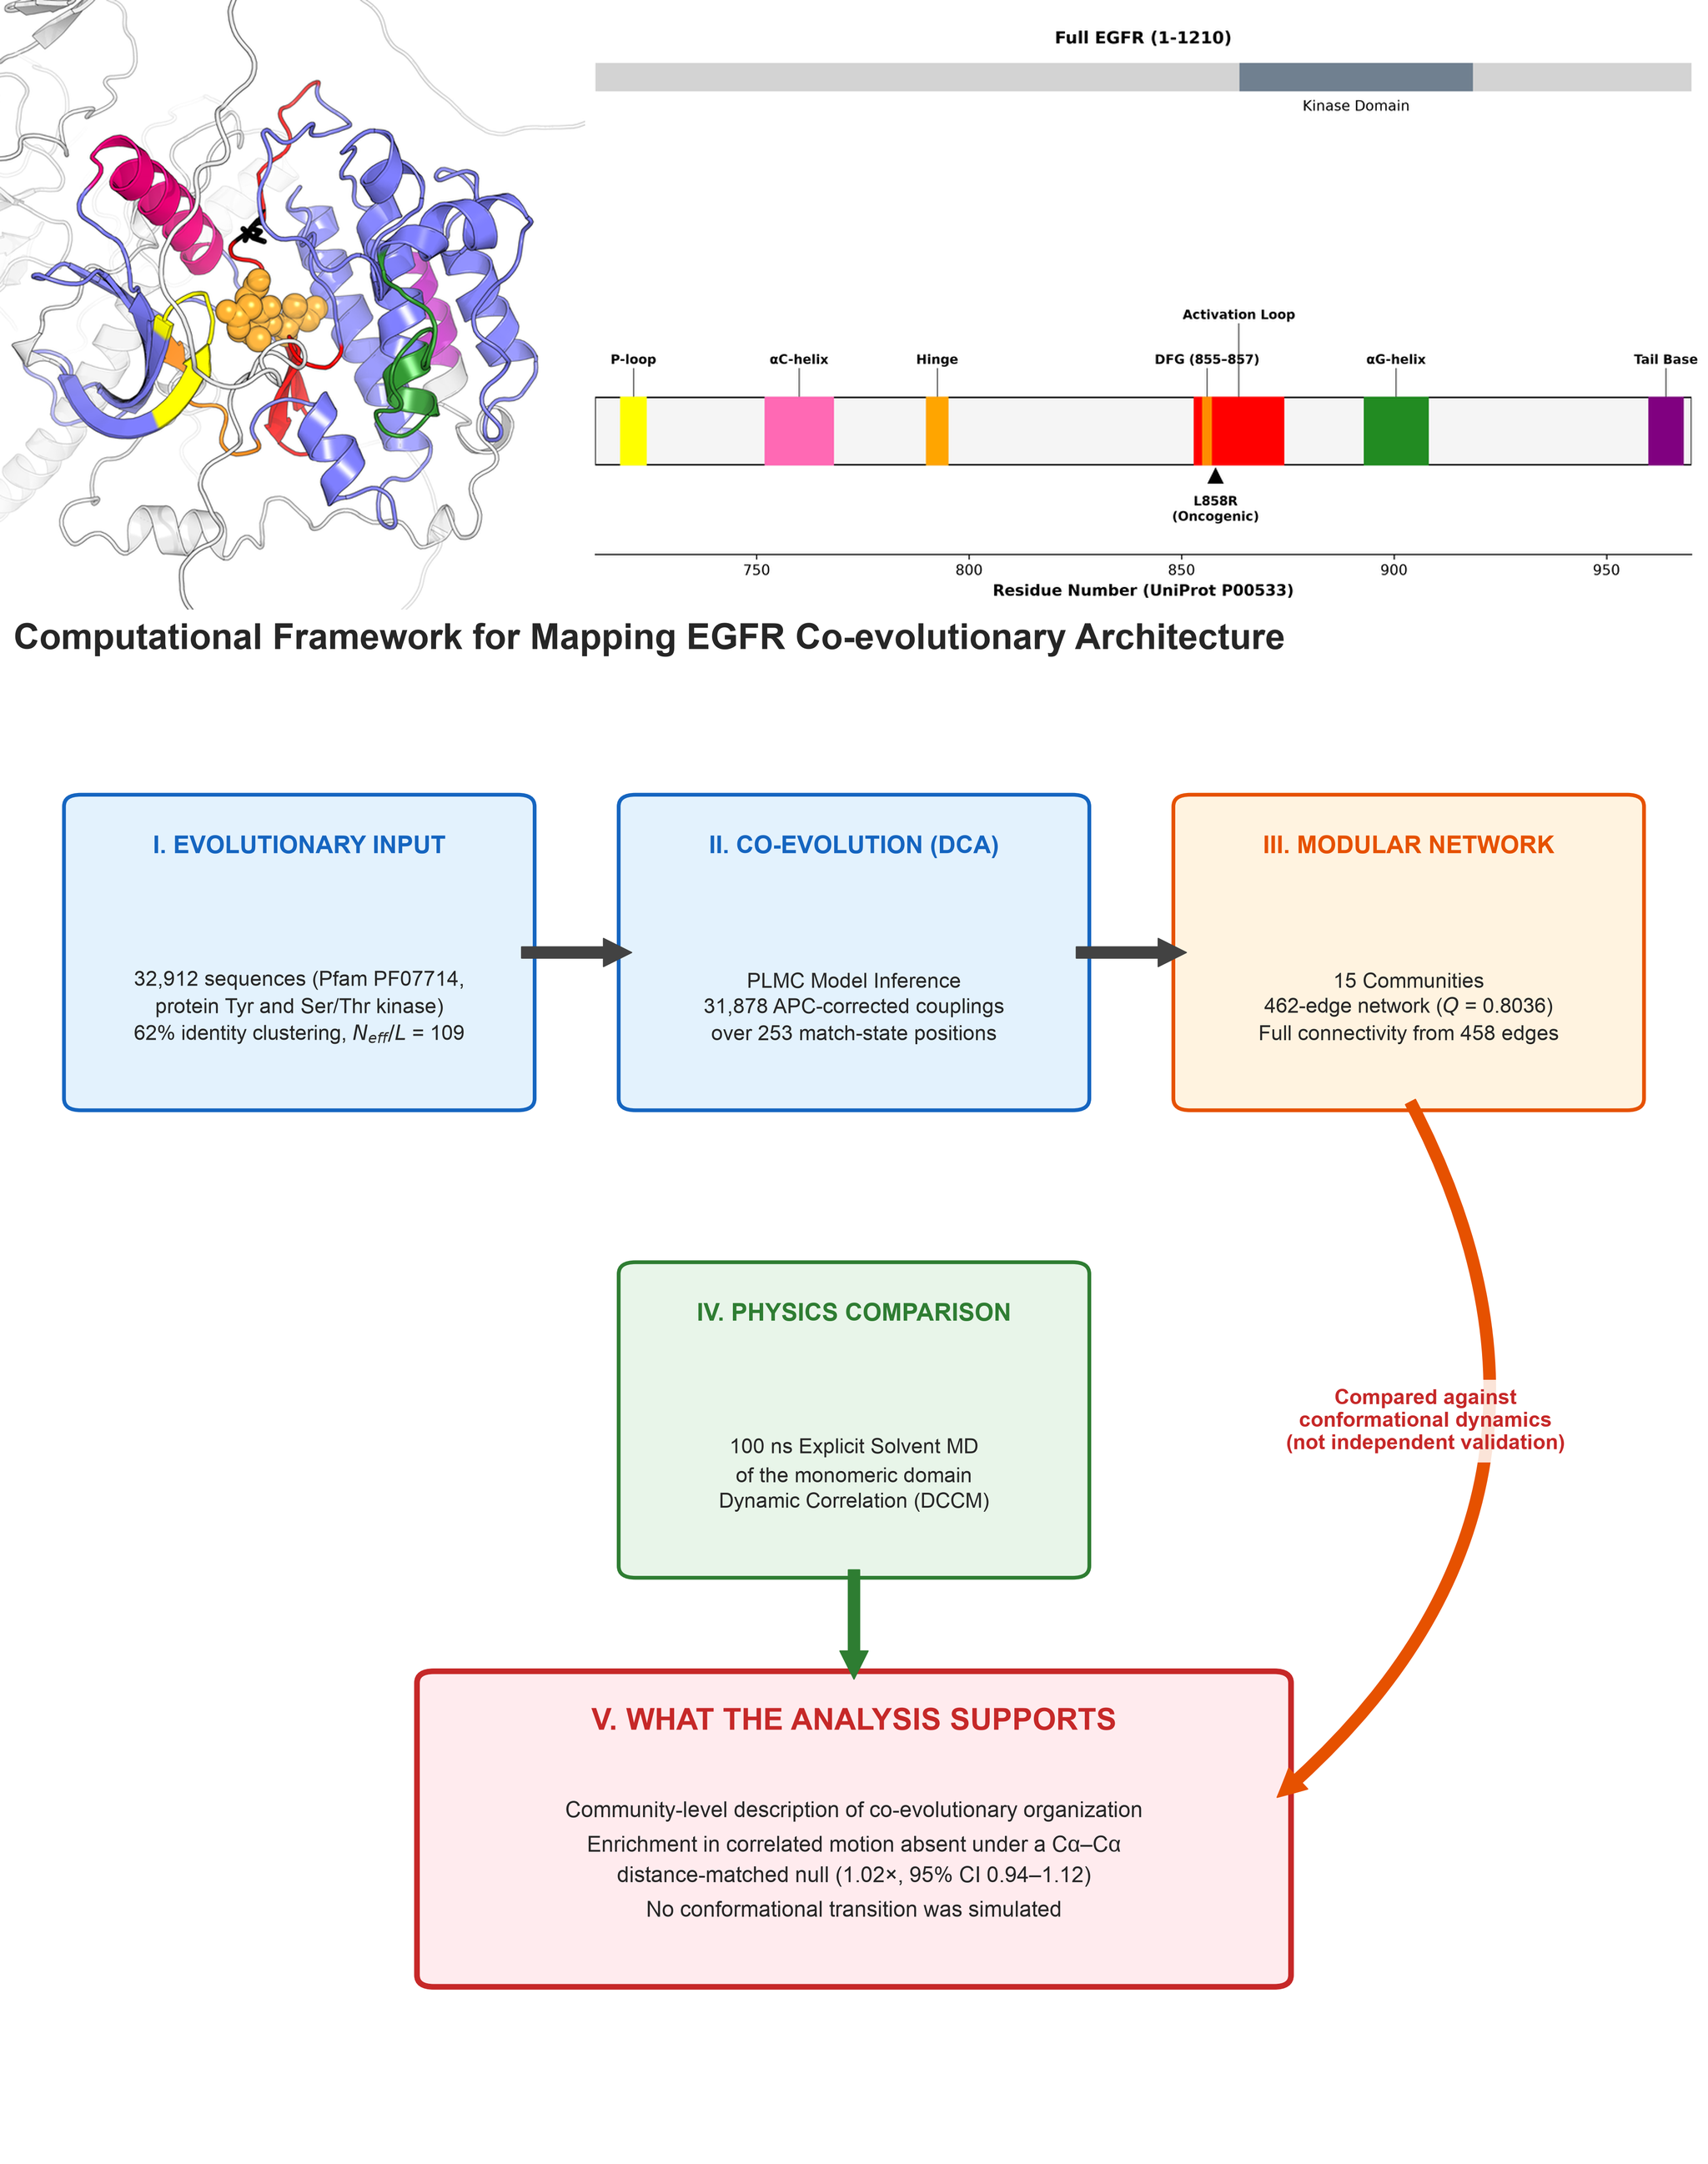
\includegraphics[width=15cm]{FIGURE_1_overview.png}
\end{center}
\caption{Framework for mapping co-evolutionary architecture in the EGFR kinase domain. \textbf{(A)} Structural architecture of the human EGFR kinase domain. 3D representation based on the AlphaFold2 model (UniProt P00533), highlighting functional motifs: the P-loop (yellow), \textalpha{}C-helix (pink), hinge region (orange), and activation loop (red). The \textalpha{}I-helix/tail base is shown in purple. \textbf{(B)} Domain architecture and clinical context. Linear schematic of the 1,210-residue receptor identifying the catalytic domain (712\textendash 968) and the location of the oncogenic L858R mutation (black star). The DFG motif is D855\textendash F856\textendash G857. \textbf{(C)} Computational pipeline. Schematic of the analysis workflow. An alignment of 32,912 sequences from Pfam family PF07714 (protein tyrosine and serine/threonine kinase; $N_{\mathrm{eff}}/L = 109$) supports two parallel analyses: pairwise statistical modeling (PLMC) followed by topological percolation analysis, which yields the community partition (boxes II--III), and statistical coupling analysis of the same positions, which yields the sector decomposition (box IV). The pairwise couplings are then assessed against molecular dynamics (box V) and against a conformational ensemble of all solved EGFR kinase-domain structures (box VI). Box VII states the inferences the combined analysis supports; all values shown are reported with their controls in Sections 2.8 and~\ref{sec:sca}.}
\label{fig:overview}
\end{figure}

\begin{figure}[h!]
\begin{center}
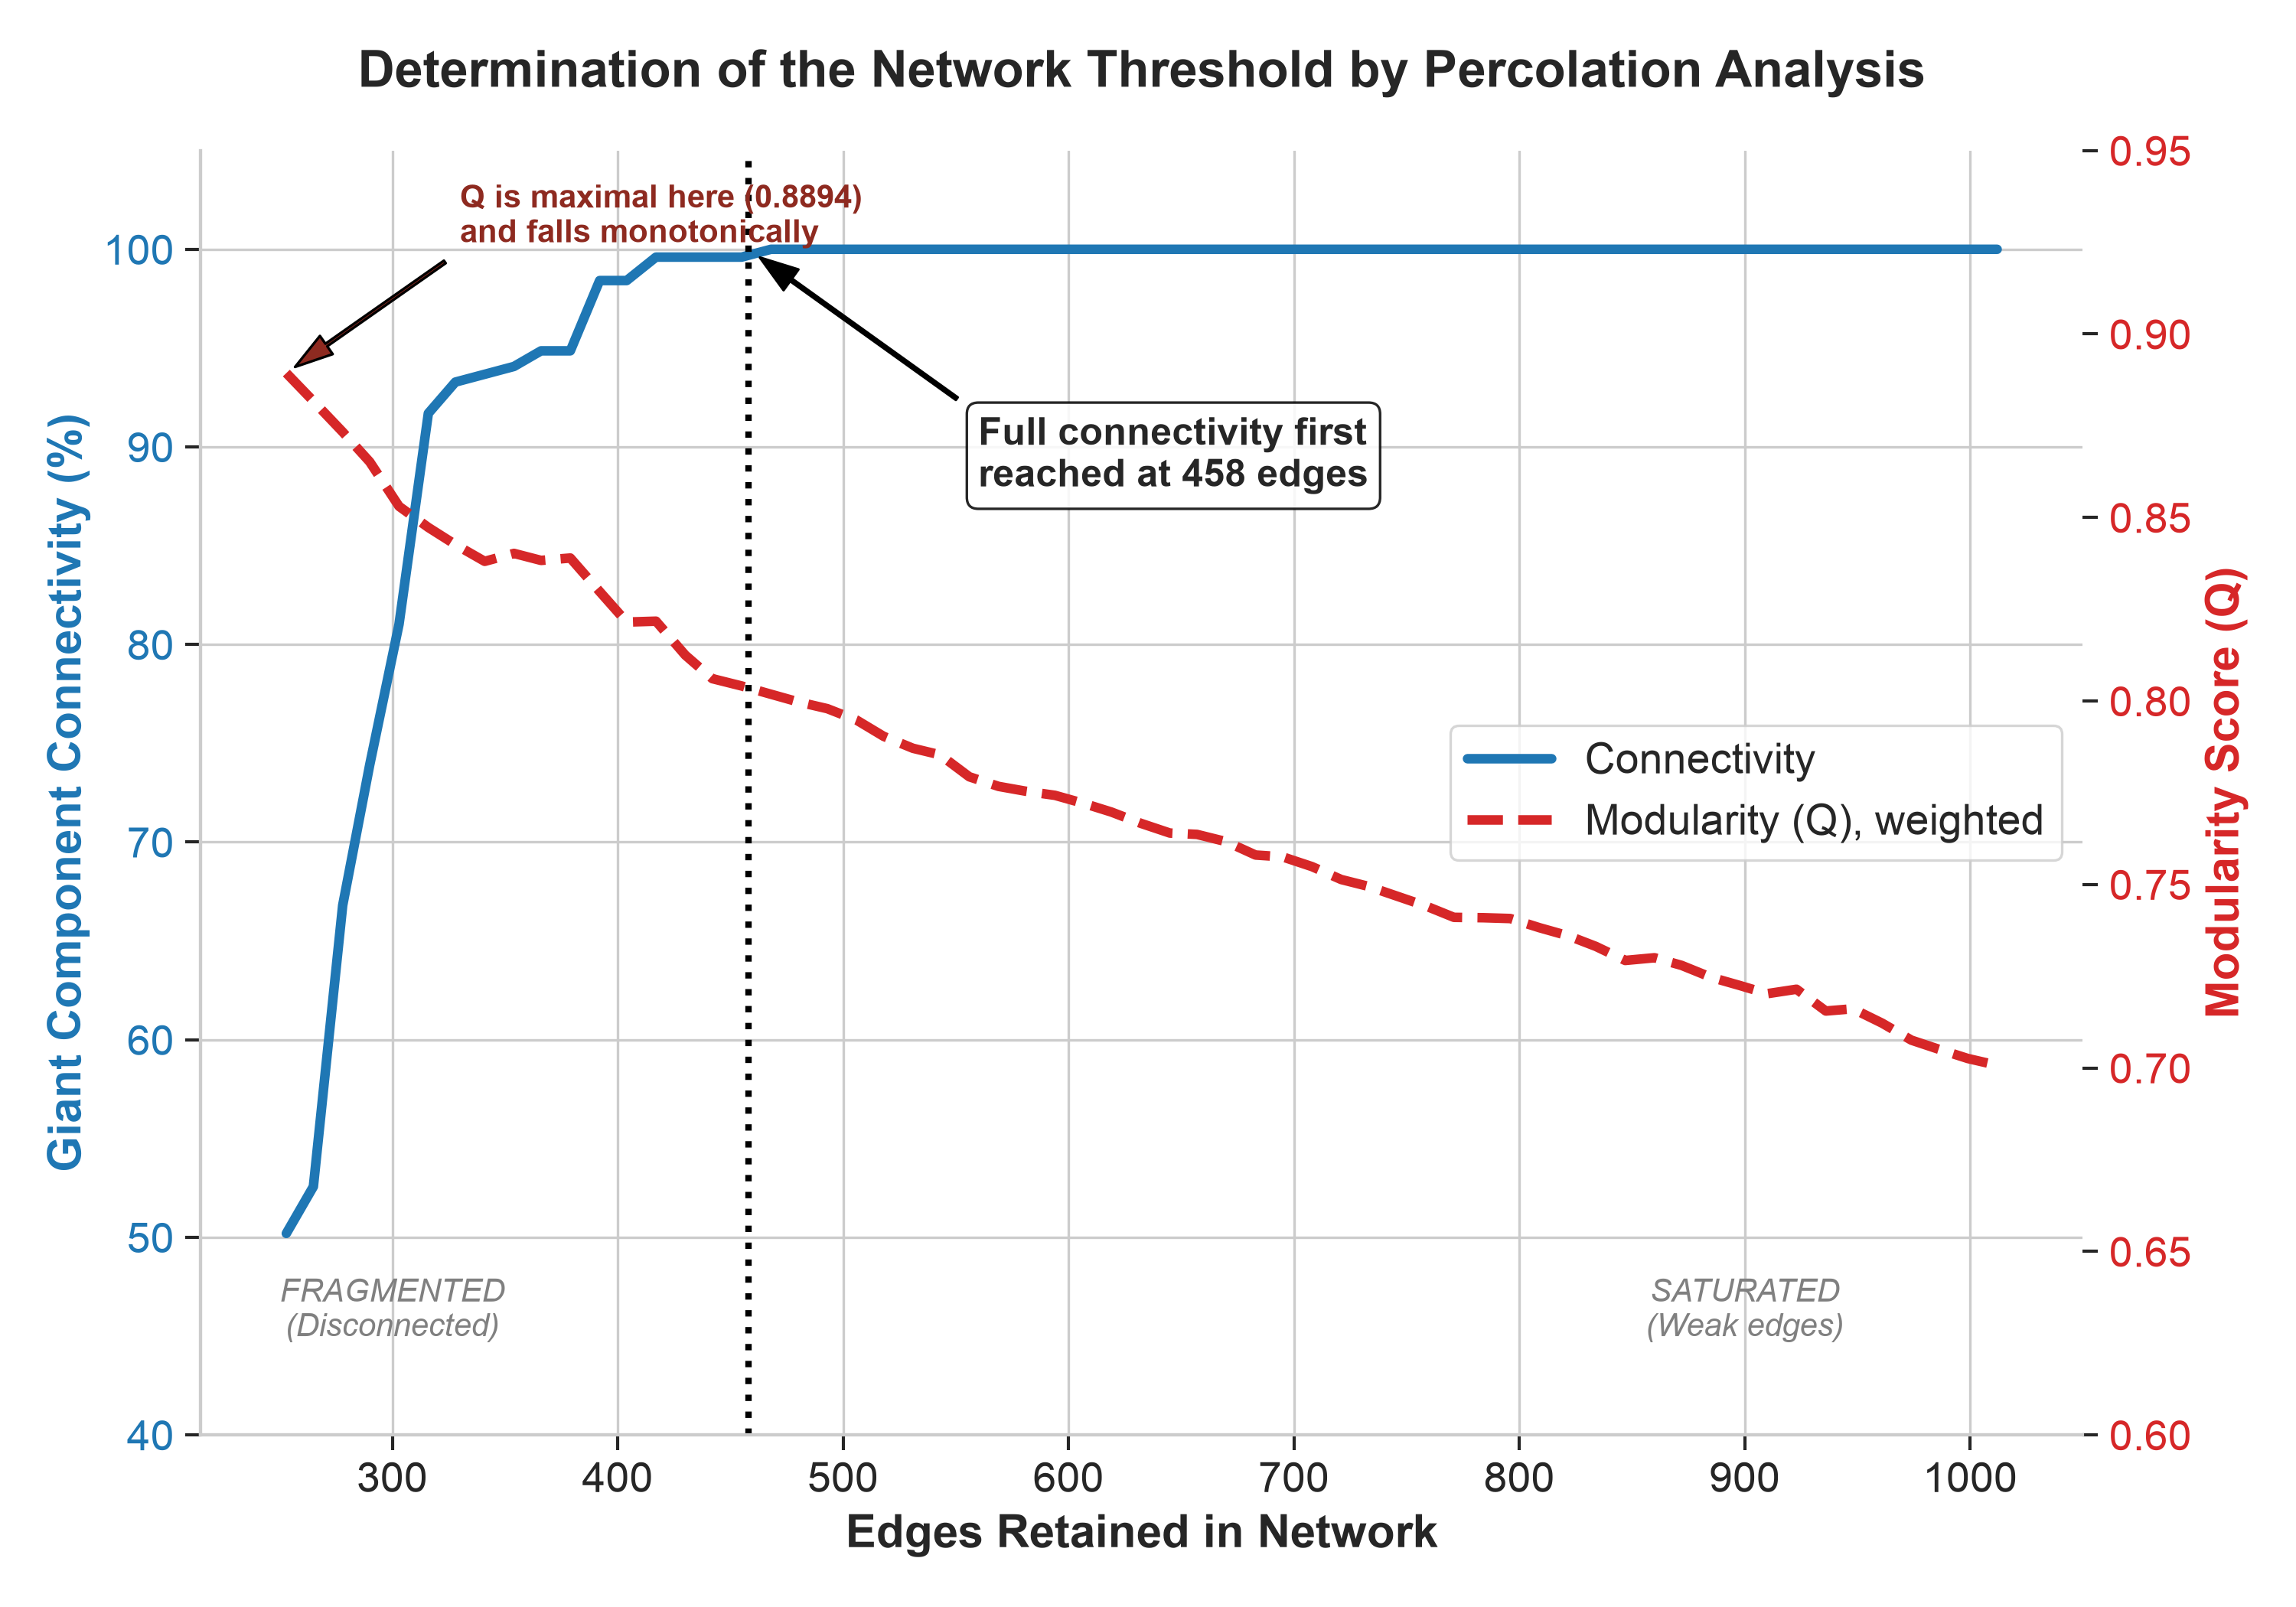
\includegraphics[width=13cm]{FIGURE_2_percolation.png}
\end{center}
\caption{Determination of the network threshold by percolation analysis. Connectivity of the largest connected component (left axis, as a percentage of the 253 analyzable residues) and modularity $Q$ of the weighted Louvain partition (right axis) as a function of the number of edges retained. Full connectivity is first achieved at 458 edges; the 462-edge network used for all downstream analyses is marked. Modularity is maximal at the lowest density tested ($Q = 0.8894$ at 253 edges, 21 communities) and decreases monotonically as edges are added, so the selected threshold is the minimum density compatible with full connectivity and not a modularity optimum. The number of communities detected over the $\pm$10\% window around the selected threshold (404\textendash 506 edges) varies between 14 and 16.}
\label{fig:percolation}
\end{figure}

\begin{figure}[h!]
\begin{center}
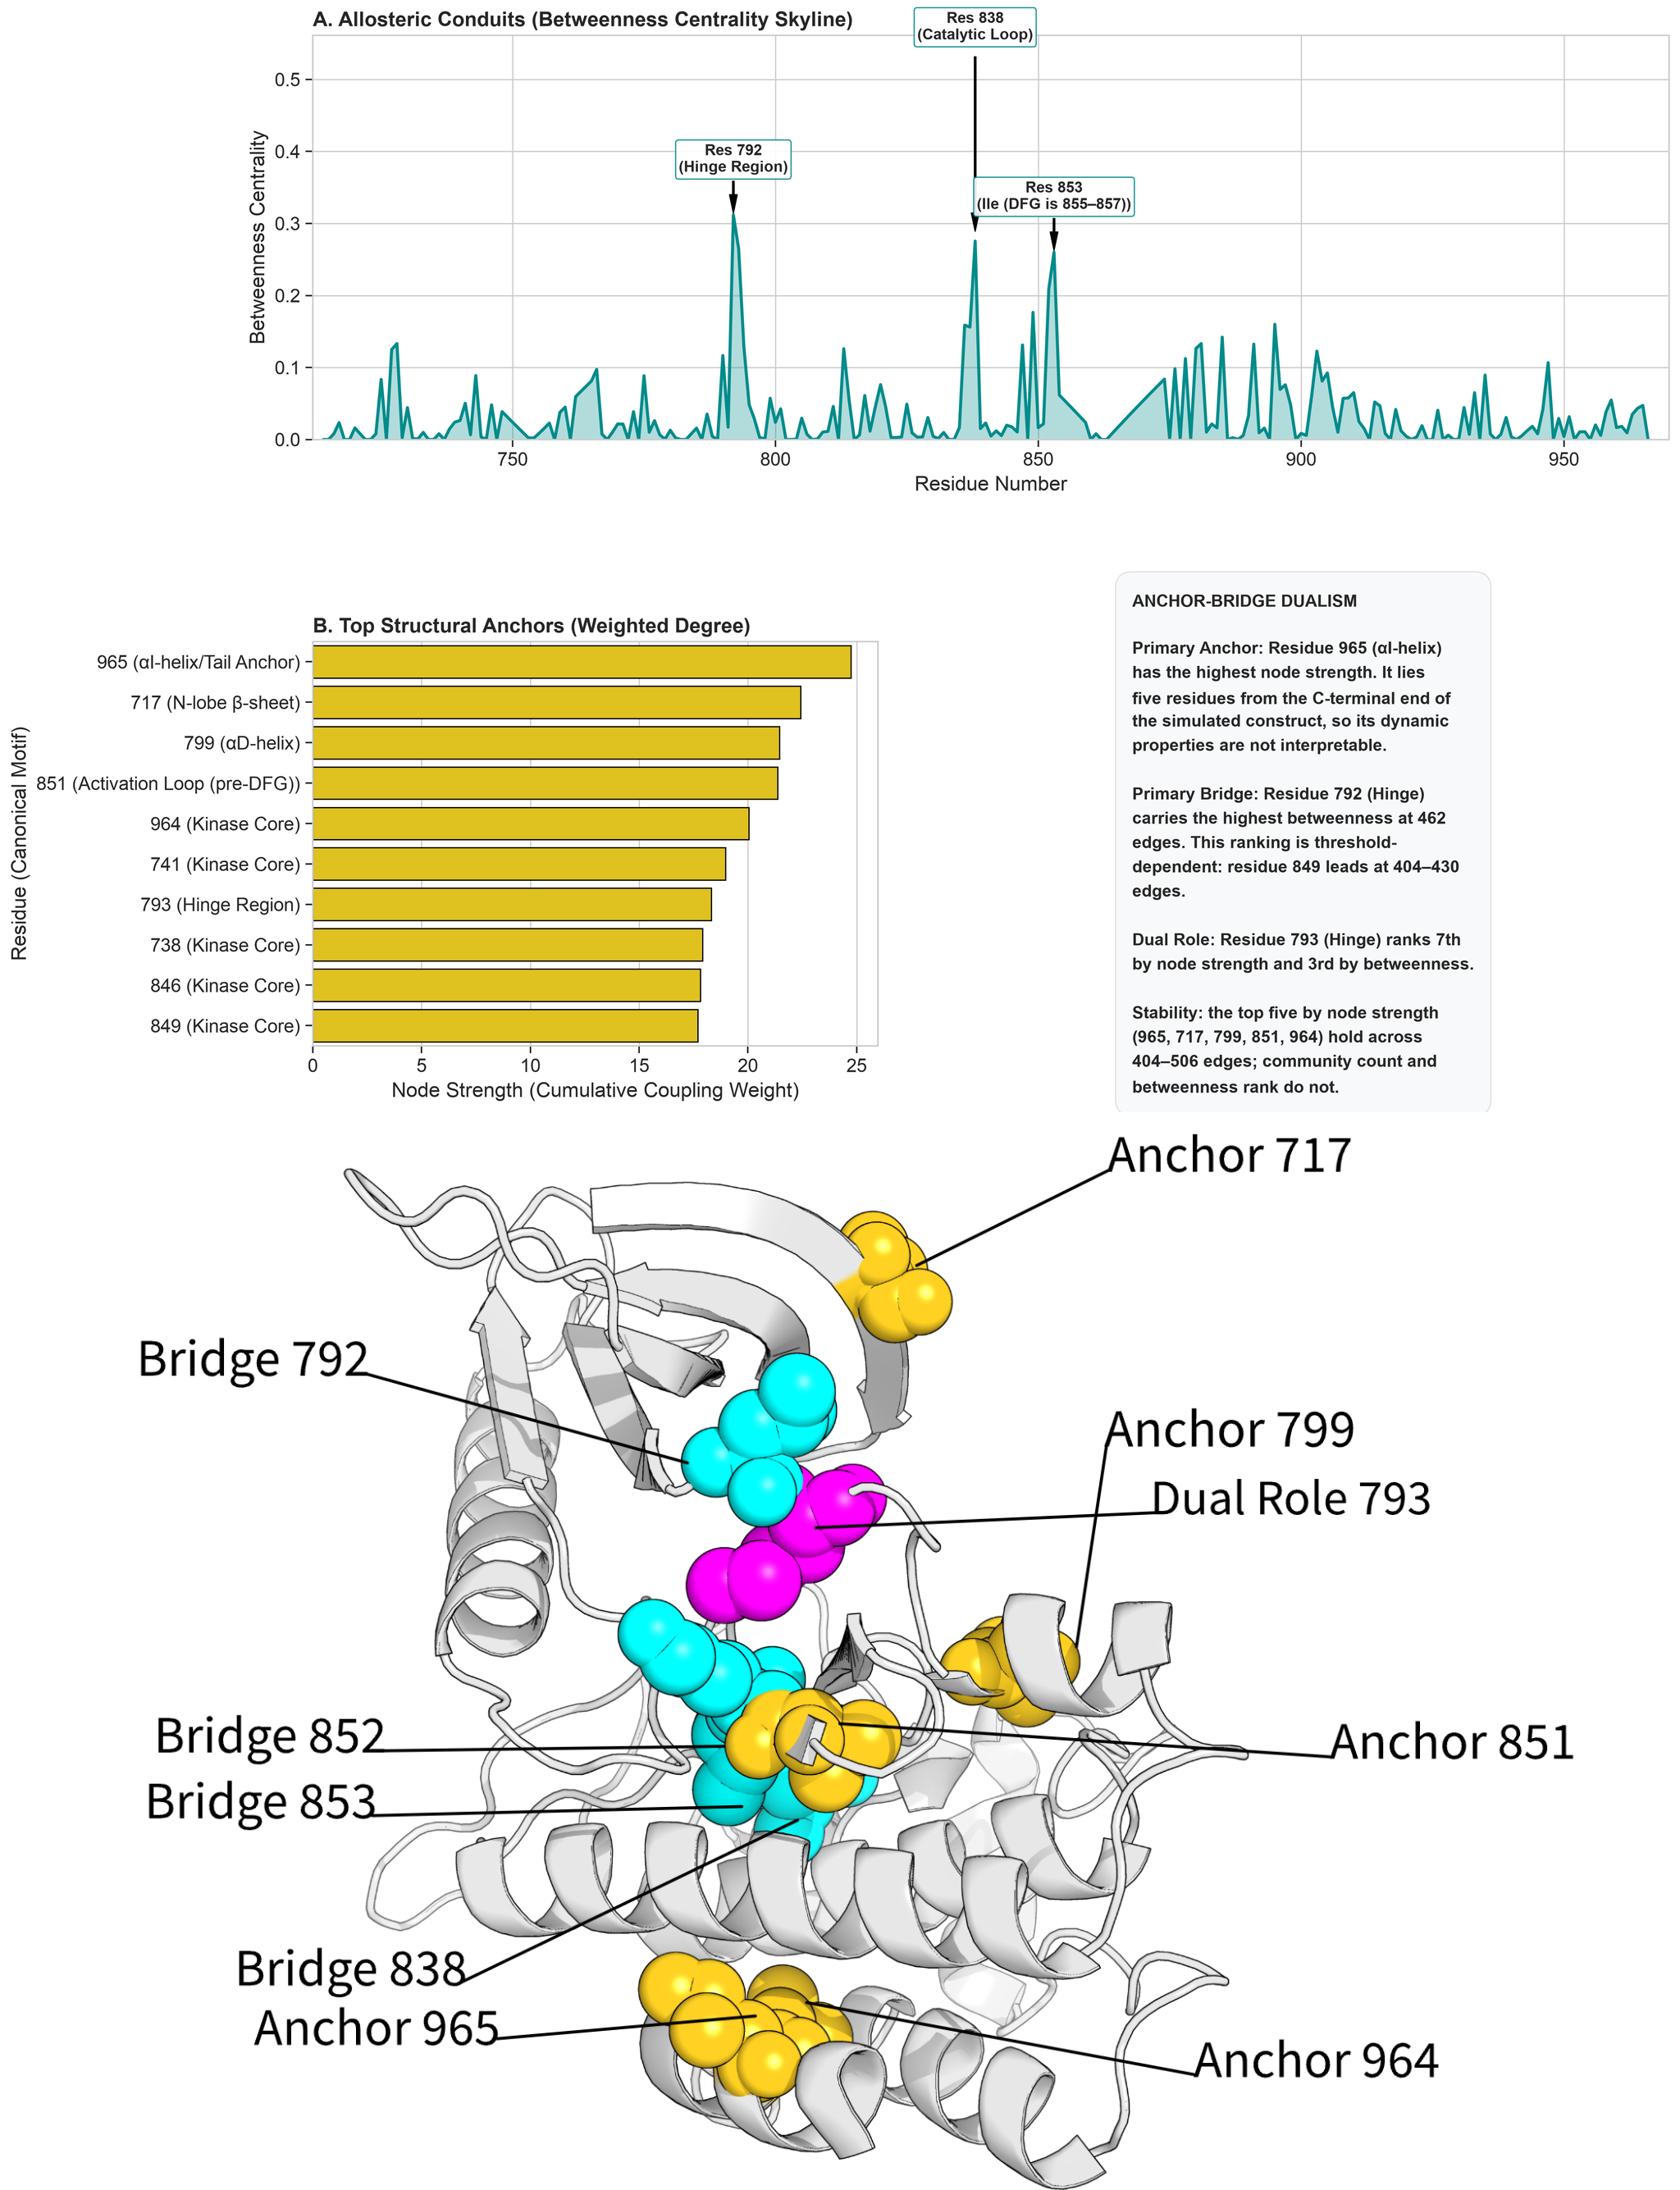
\includegraphics[width=13cm]{FIGURE_3_centrality.png}
\end{center}
\caption{Anchor\textendash Bridge Dualism in Network Topology. \textbf{(A)} Allosteric Conduit Profile. Betweenness centrality skyline identifying residues that serve as global bottlenecks for information flow. Primary peaks occur at the hinge (792, 793) and the catalytic loop (838). Residue 853 is isoleucine; the DFG motif is D855\textendash F856\textendash G857. \textbf{(B)} Top-ranked residues by node strength (weighted degree). Residue 965 has the highest node strength in the network; it lies five residues from the C-terminal end of the simulated construct, so its dynamic properties are not interpretable (Section 2.5). The top five by node strength are stable across the 404\textendash 506 edge range, whereas the betweenness ranking in (A) is not. \textbf{(C)} Structural mapping contrasting high node-strength residues (gold spheres) with high-betweenness residues (cyan spheres).}
\label{fig:centrality}
\end{figure}

\begin{figure}[h!]
\begin{center}
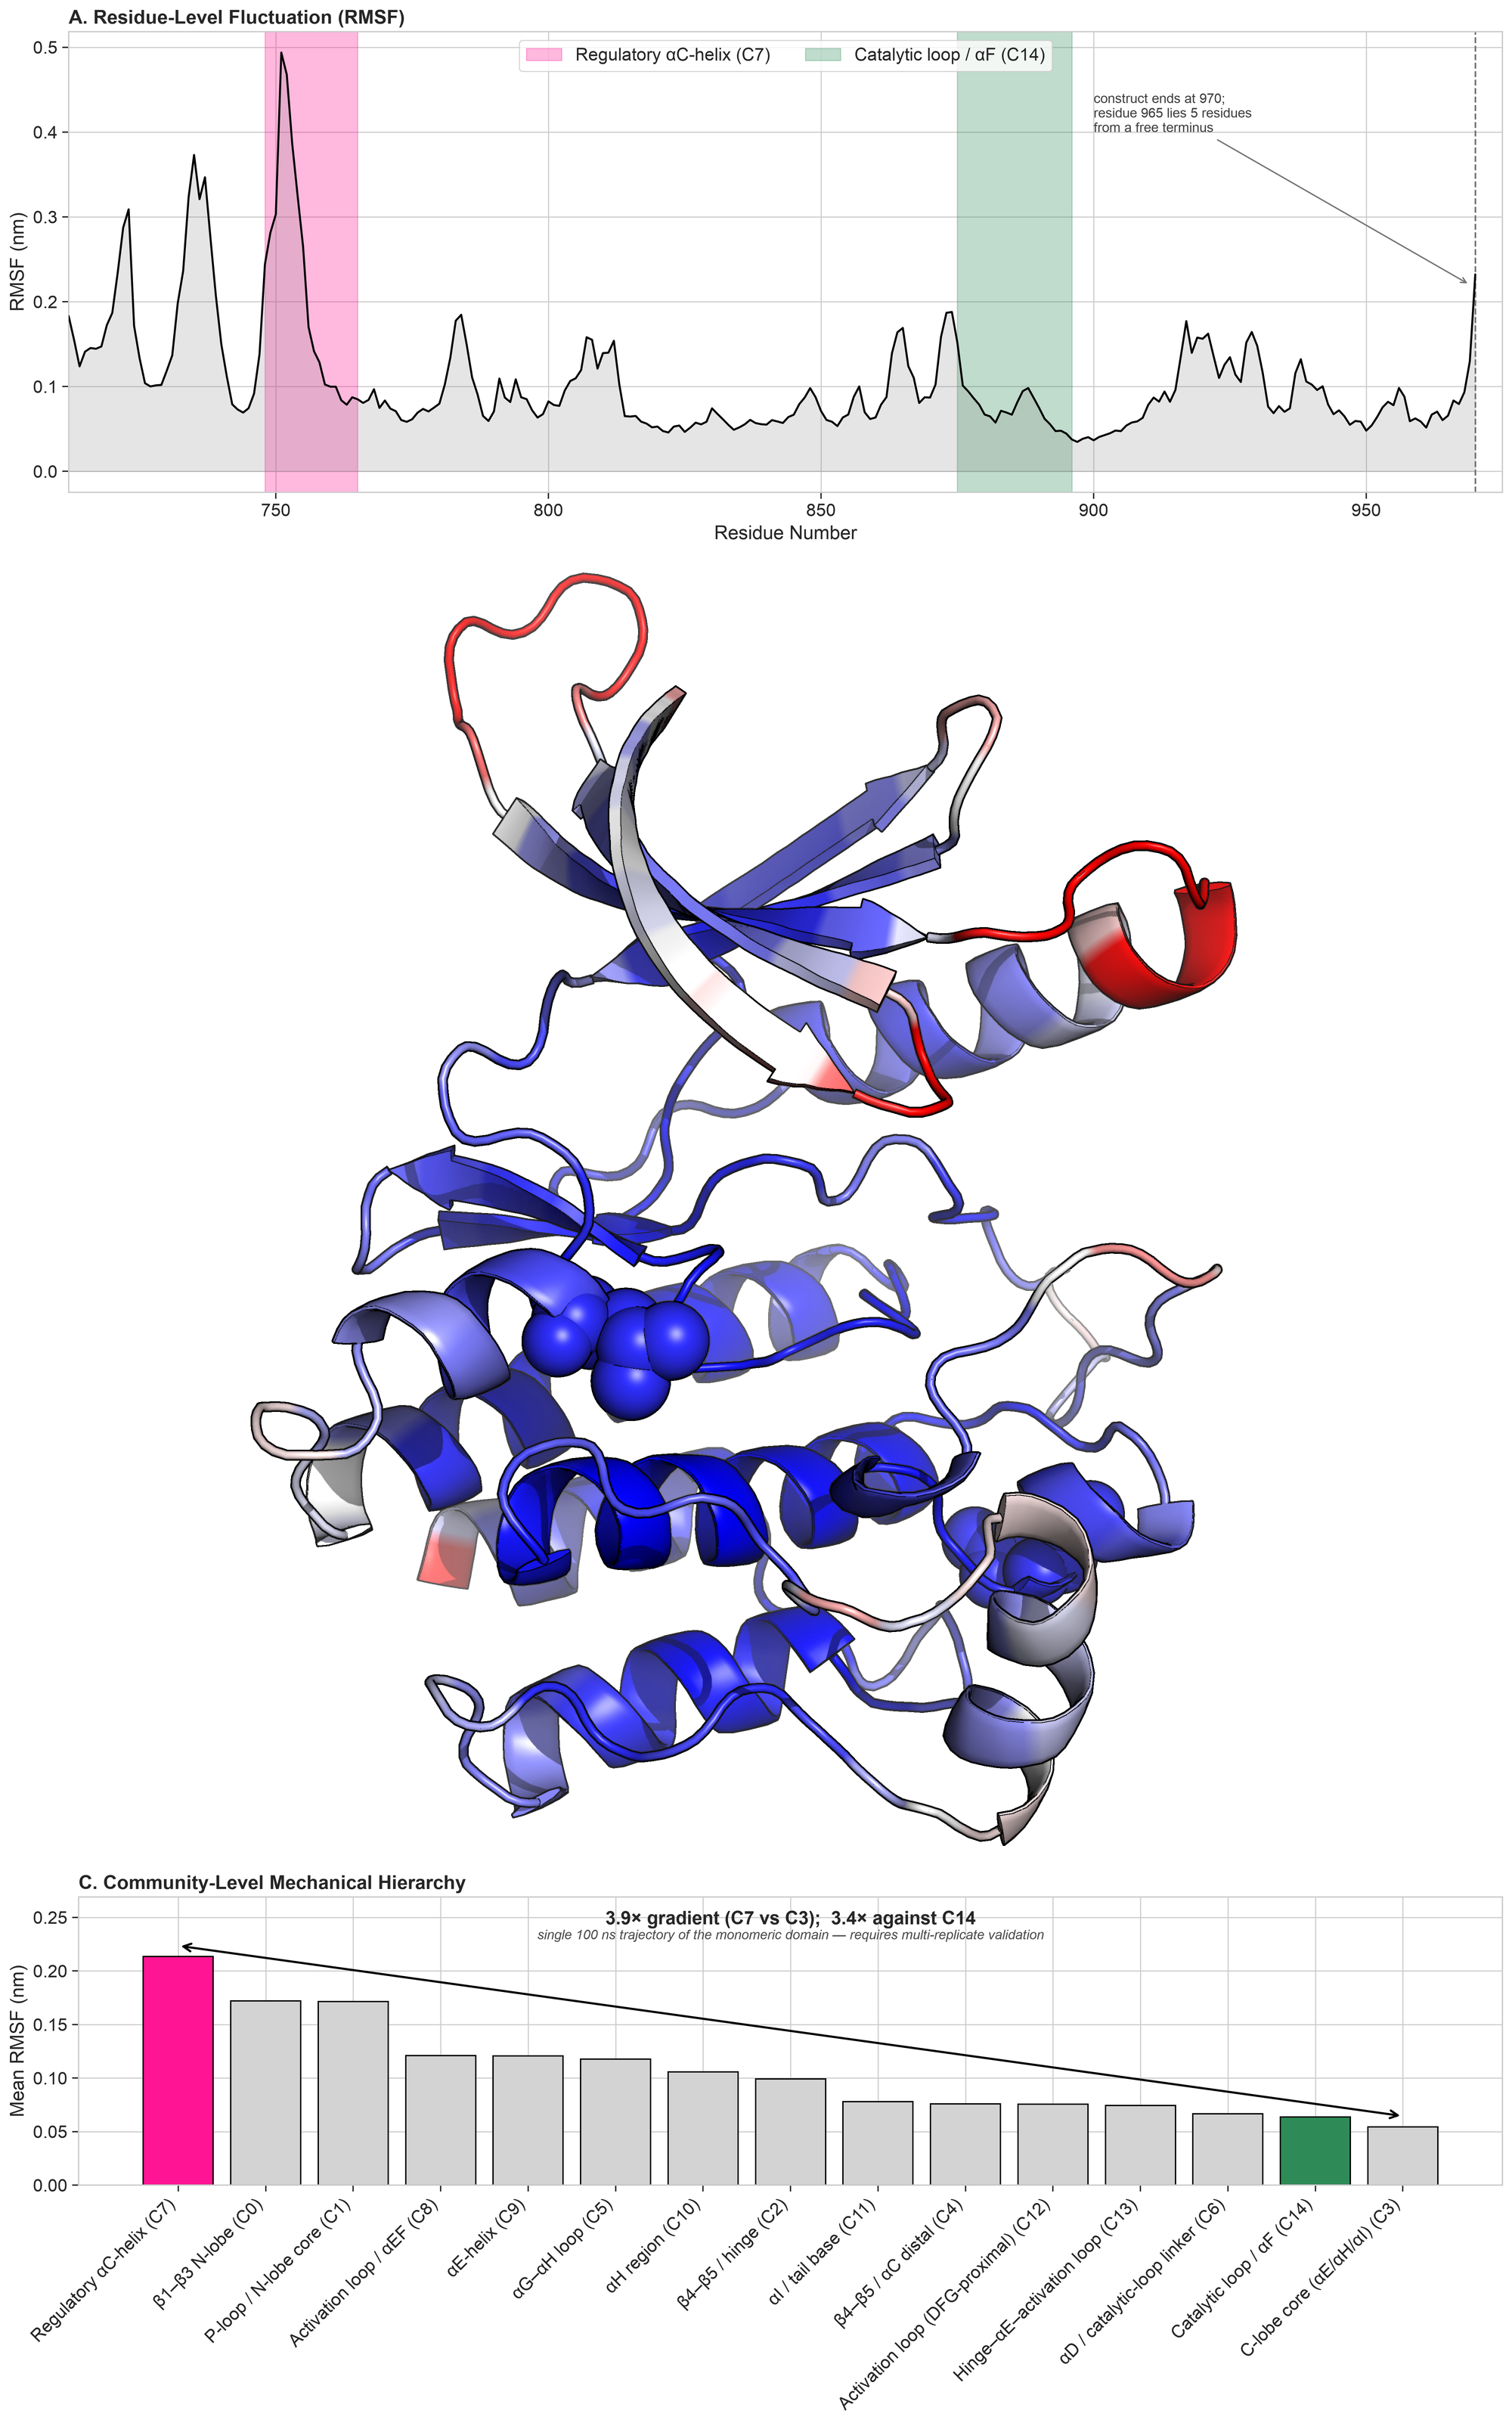
\includegraphics[width=9cm]{FIGURE_4_rmsf.png}
\end{center}
\caption{Mechanical Hierarchy and the Global Rigidity Gradient. \textbf{(A)} Residue-Level Fluctuation Profile (RMSF). Local fluctuations derived from 100 ns of MD simulation. The three largest peaks are residues 751\textendash 753 (0.494, 0.468 and 0.386~nm) at the \textbeta{}3--\textalpha{}C junction, followed by residues 734\textendash 737 in the N-lobe \textbeta{}-sheet; the activation loop is not among the high-fluctuation regions in this trajectory (maximum 0.188~nm at residue 874). Both flexible regions recur in every replicate and the activation loop is never among the eight most mobile positions, but the rank order of individual peaks within those regions is trajectory-specific (Section~\ref{sec:replicates}). \textbf{(B)} Structural Rigidity Map. AlphaFold model colored by a blue-to-red spectrum representing the rigidity gradient. The rigid \textalpha{}F-helix core provides a stable scaffold for the more mobile N-lobe and \textalpha{}C-helix region. \textbf{(C)} Module-level mechanical hierarchy. Mean RMSF per evolutionary community. The gradient between the most mobile community (Community 7, 0.2135 nm) and the most rigid (Community 3, 0.0545 nm) is 3.9-fold; the ratio against Community 14 (0.0636 nm) is 3.4-fold. Values derive from replicate 1 of five 100 ns trajectories of the monomeric domain. The ordering is reproduced in all five replicates --- Community 7 most mobile, Community 3 most rigid --- while the magnitude of the gradient spans 2.8--4.0-fold across replicates (Section~\ref{sec:replicates}).}
\label{fig:rmsf}
\end{figure}

\begin{figure}[h!]
\begin{center}
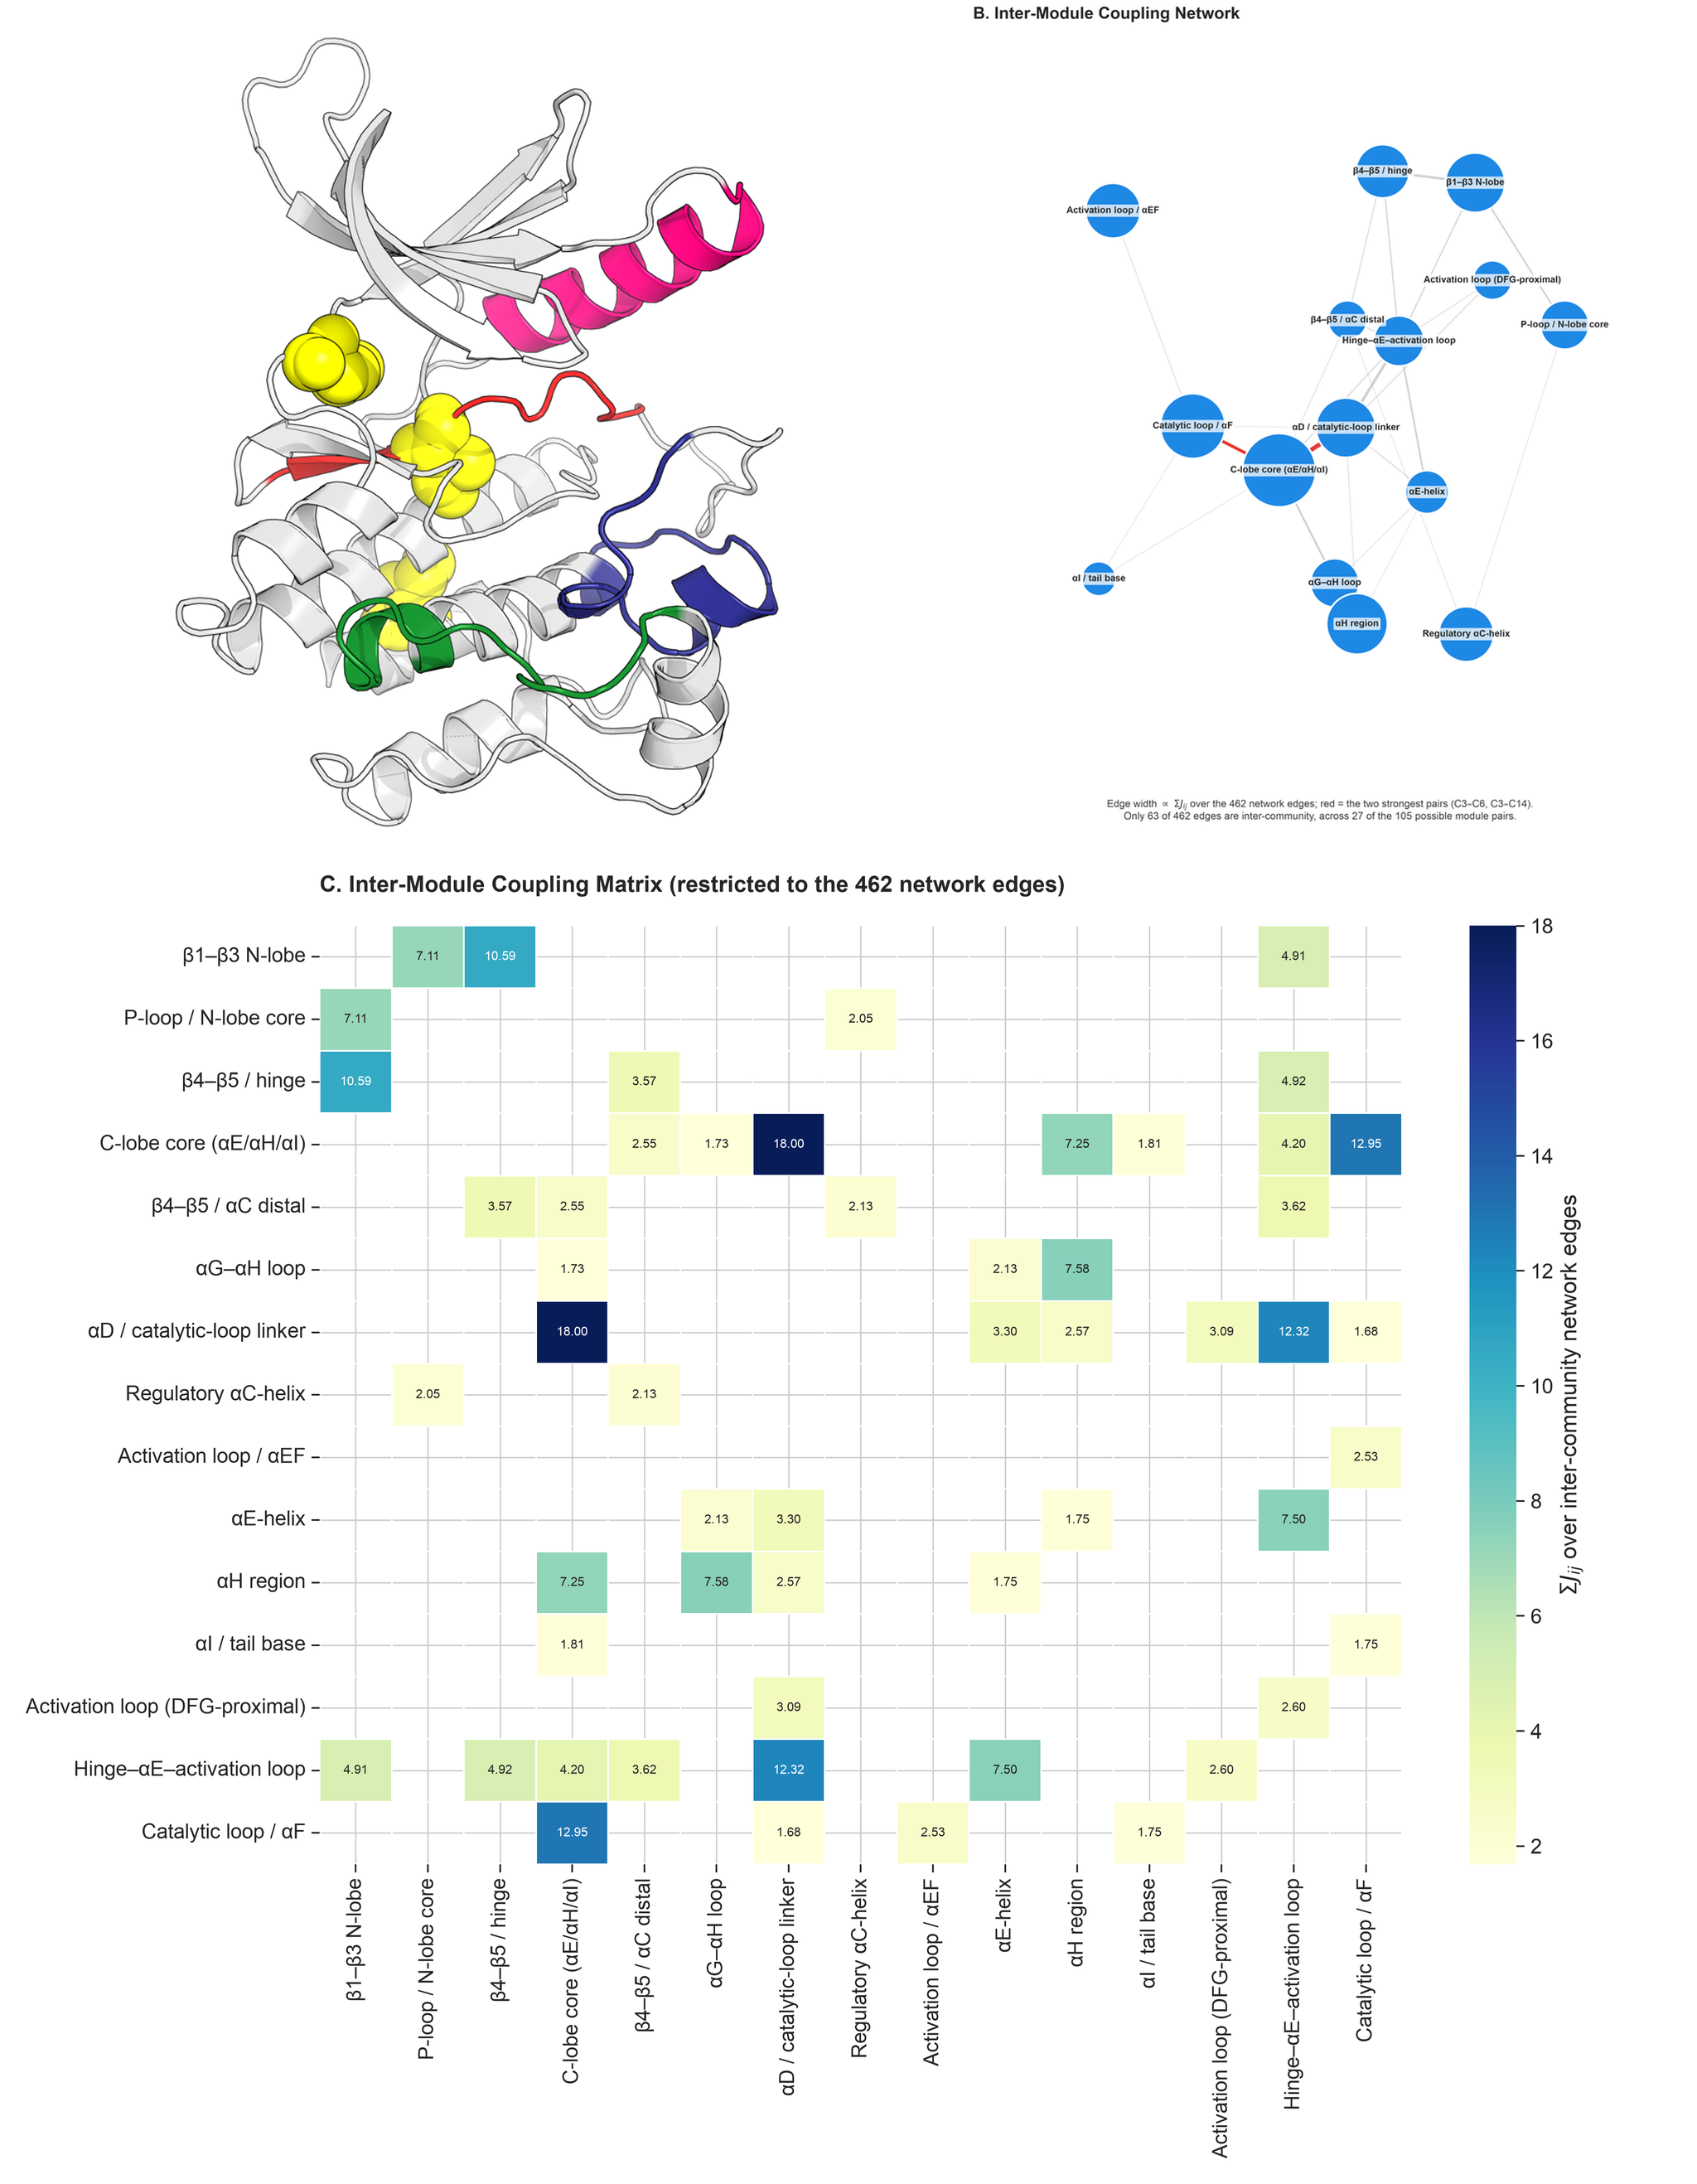
\includegraphics[width=13cm]{FIGURE_5_flux.png}
\end{center}
\caption{Modular organization of the kinase domain. \textbf{(A)} 3D functional community map. Partitioning of the domain into 15 communities at the selected network threshold. \textbf{(B)} Inter-module graph. Node size is proportional to residue count; edge thickness represents cumulative inter-module coupling over the 462 network edges. Only 63 of the 462 edges cross community boundaries, distributed across 27 of the 105 possible module pairs. \textbf{(C)} Inter-module coupling matrix. Because the coupling scores are average-product-corrected and signed with a mean near zero, the cumulative sum over all $|A|\times|B|$ residue pairs is negative for 75 of the 105 module pairs and is negatively correlated with the number of pairs ($r=-0.33$); it is shown here for completeness but is not used to rank pathways. Ranked instead by coupling over the network edges, the strongest pairs are Community 3\textendash Community 6 (8 edges, $\sum J_{ij}=18.01$) and Community 3\textendash Community 14 (7 edges, $\sum J_{ij}=12.95$). See Section~\ref{sec:flux}.}
\label{fig:flux}
\end{figure}

\begin{figure}[h!]
\begin{center}
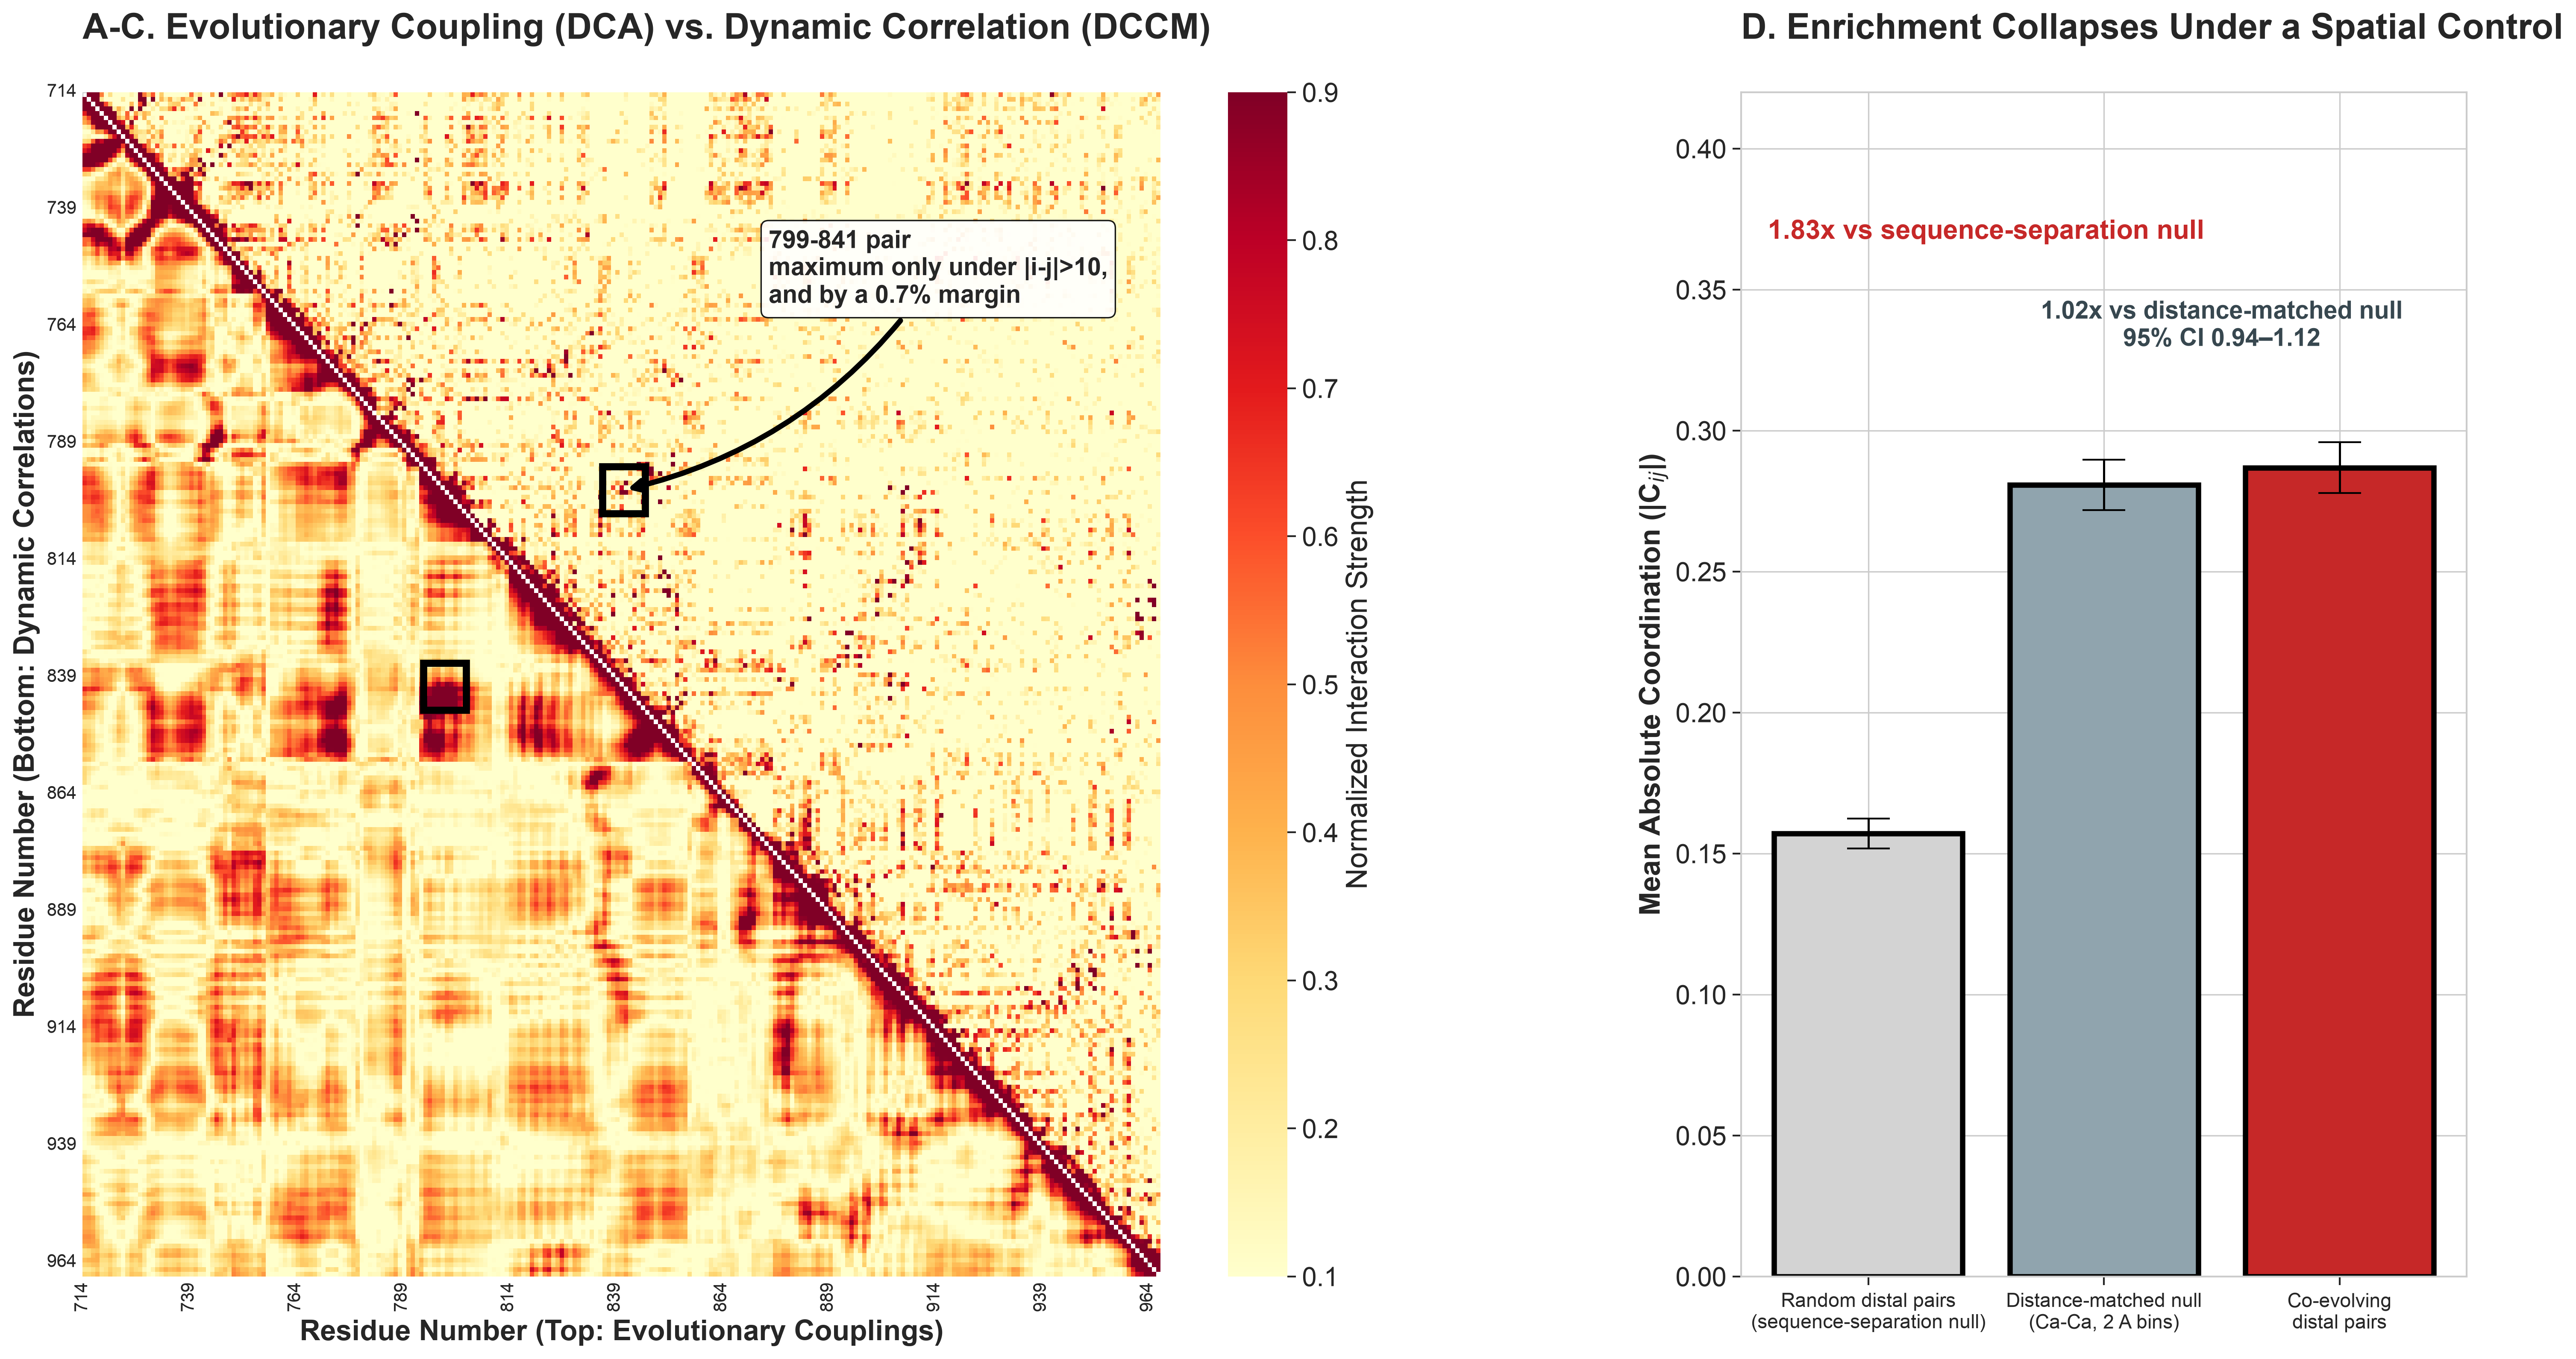
\includegraphics[width=13cm]{FIGURE_6_dccm.png}
\end{center}
\caption{Co-evolutionary coupling against dynamic correlation. \textbf{(A--C)} Mirror heatmap comparing the normalized evolutionary coupling matrix (DCA, upper triangle) with the absolute dynamic cross-correlation matrix (DCCM, lower triangle). Black boxes mark the 799\textendash 841 pair, which maximizes the product of coupling strength and absolute dynamic correlation under an $|i-j|>10$ filter, though by a margin of 0.7\% over the runner-up; under the $|i-j|>5$ filter used elsewhere the maximum is instead pair 717-725 (Section 2.7). \textbf{(D)} Enrichment in correlated motion of the 500 most strongly co-evolving distal pairs against two null models, each of 500 pairs. Against a null matched only on sequence separation the enrichment is 1.83-fold (nominal $p = 1.1\times10^{-33}$; the nominal value treats pairs as independent, which they are not --- see Section 2.8), reproducing the previously reported value. Against a null additionally matched on C\textalpha{}--C\textalpha{} distance in 2~\AA{} bins the enrichment is 1.02-fold (bootstrap 95\% CI 0.94\textendash 1.12; $p \approx 0.5$), indicating that the apparent correspondence is accounted for by three-dimensional proximity. Error bars are bootstrap 95\% confidence intervals. Panels show replicate 1; both results reproduce across five independent trajectories, 1.45\textendash 1.88-fold under the sequence-separation null and 0.95\textendash 1.02-fold under the distance-matched null (Figure~\ref{fig:replicates}, Section~\ref{sec:replicates}).}
\label{fig:dccm}
\end{figure}

\begin{figure}[h!]
\begin{center}
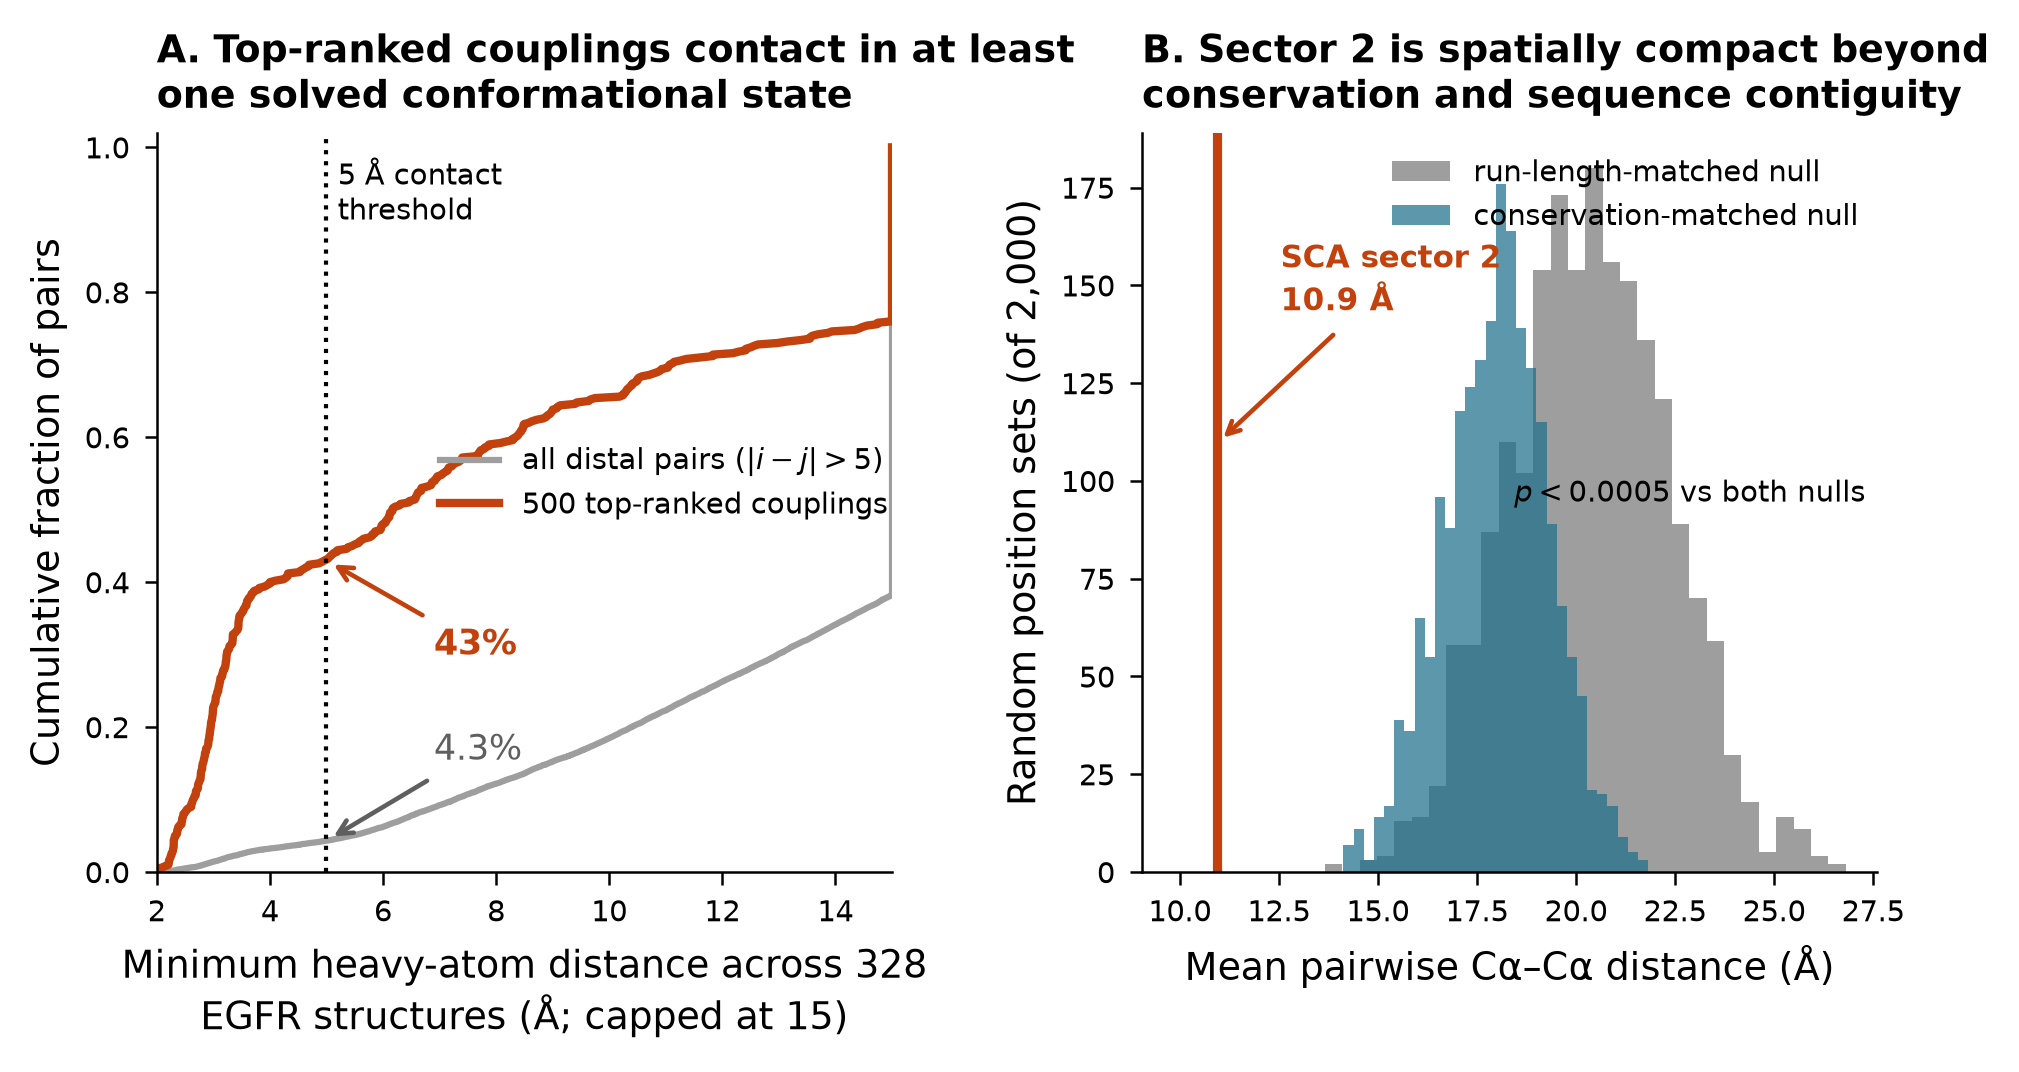
\includegraphics[width=15cm]{FIGURE_7_sectors.png}
\end{center}
\caption{Conformational-ensemble contact composition of the co-evolving set, and collective sector organization. \textbf{(A)} Cumulative distribution of the minimum heavy-atom distance across a conformational ensemble of 537 chains from 328 EGFR structures, for the 500 top-ranked co-evolving pairs and for all distal pairs ($|i-j|>5$; $n = 30{,}628$). Distances are capped at 15~\AA{}, so each curve plateaus below 1.0 at the right-hand limit. 43.0\% of the top-ranked pairs are within 5~\AA{} in at least one solved state, against 4.3\% of all distal pairs, establishing that the set is dominated by contacts formed in some conformational state rather than by long-range couplings. \textbf{(B)} Mean pairwise C\textalpha{}--C\textalpha{} distance of SCA sector 2 (22 positions; vertical line) against two null distributions of 2,000 random position sets each. The conservation-matched null reproduces the sector's distribution over deciles of positional relative entropy; the run-length-matched null reproduces its multiset of contiguous sequence runs at random non-overlapping positions. No draw from either null reached the observed value. The sector is therefore spatially clustered beyond what its conservation profile or its sequence contiguity predicts, although its membership is itself strongly conservation-correlated (Section~\ref{sec:sca}).}
\label{fig:sectors}
\end{figure}

\begin{figure}[h!]
\begin{center}
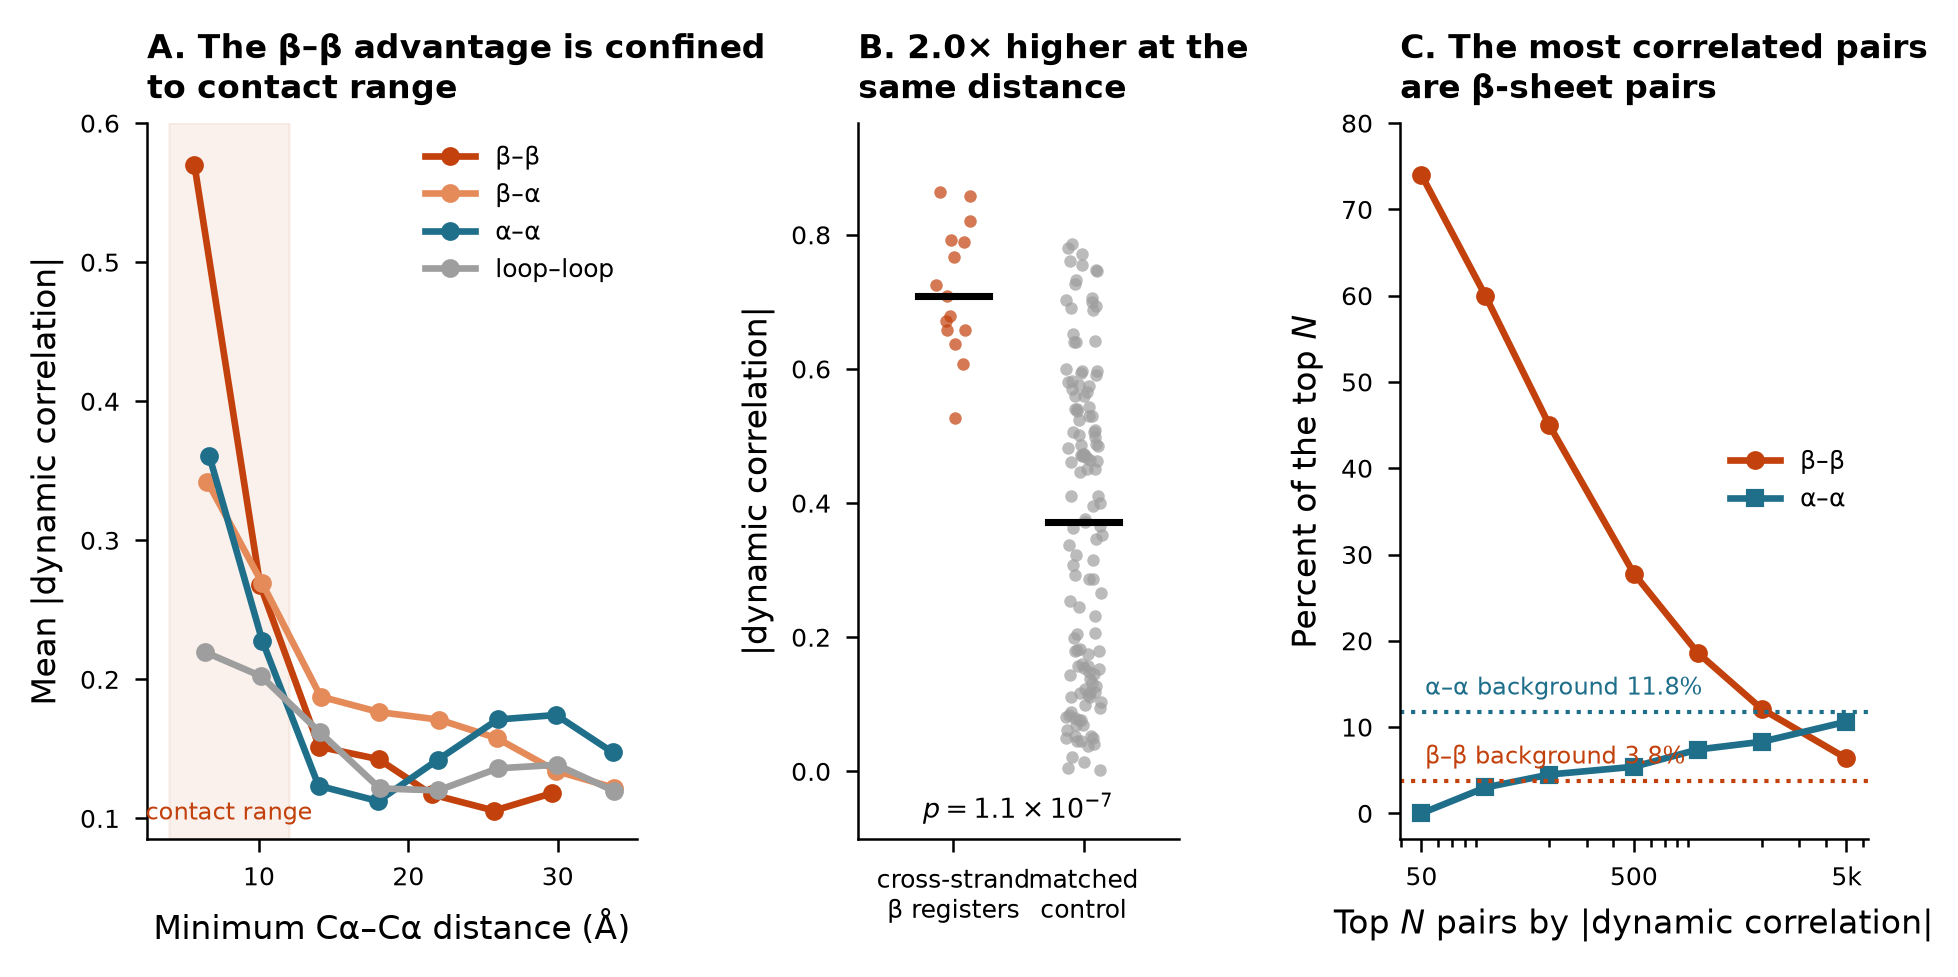
\includegraphics[width=15cm]{FIGURE_8_beta_sheet.png}
\end{center}
\caption{Correlated motion in the kinase domain follows \textbeta{}-sheet architecture. Secondary structure was assigned by DSSP over 501 frames of the production trajectory and every residue pair labelled by the secondary-structure classes of its two members; all panels use distal pairs ($|i-j|>5$, $n = 30{,}628$). \textbf{(A)} Mean absolute dynamic correlation against minimum C\textalpha{}--C\textalpha{} distance, by pairing class. \textbeta{}--\textbeta{} pairs are the most correlated class within the shaded contact range but fall below \textbeta{}--helix and helix--helix pairs beyond approximately 12~\AA{}, so the effect does not extend to long range. Bins containing fewer than 20 pairs are omitted. \textbf{(B)} The 15 cross-strand \textbeta{} registers (both members \textbeta{}-strand, backbone hydrogen-bond occupancy $\geq 0.5$, sequence separation $>4$) against the 131 pairs of other classes falling in the same 4.2--5.3~\AA{} window; horizontal bars are medians. The 1.99-fold difference is not attributable to proximity, since the two groups occupy the same distance range. \textbf{(C)} Percentage of the $N$ most strongly correlated pairs that are \textbeta{}--\textbeta{} or helix--helix, against their background frequencies among all distal pairs (dotted lines). \textbeta{}-sheet pairs dominate the top of the distribution and helical pairs are depleted.}
\label{fig:betasheet}
\end{figure}


\section*{Supplementary Material}

\begin{figure}[h!]
\begin{center}
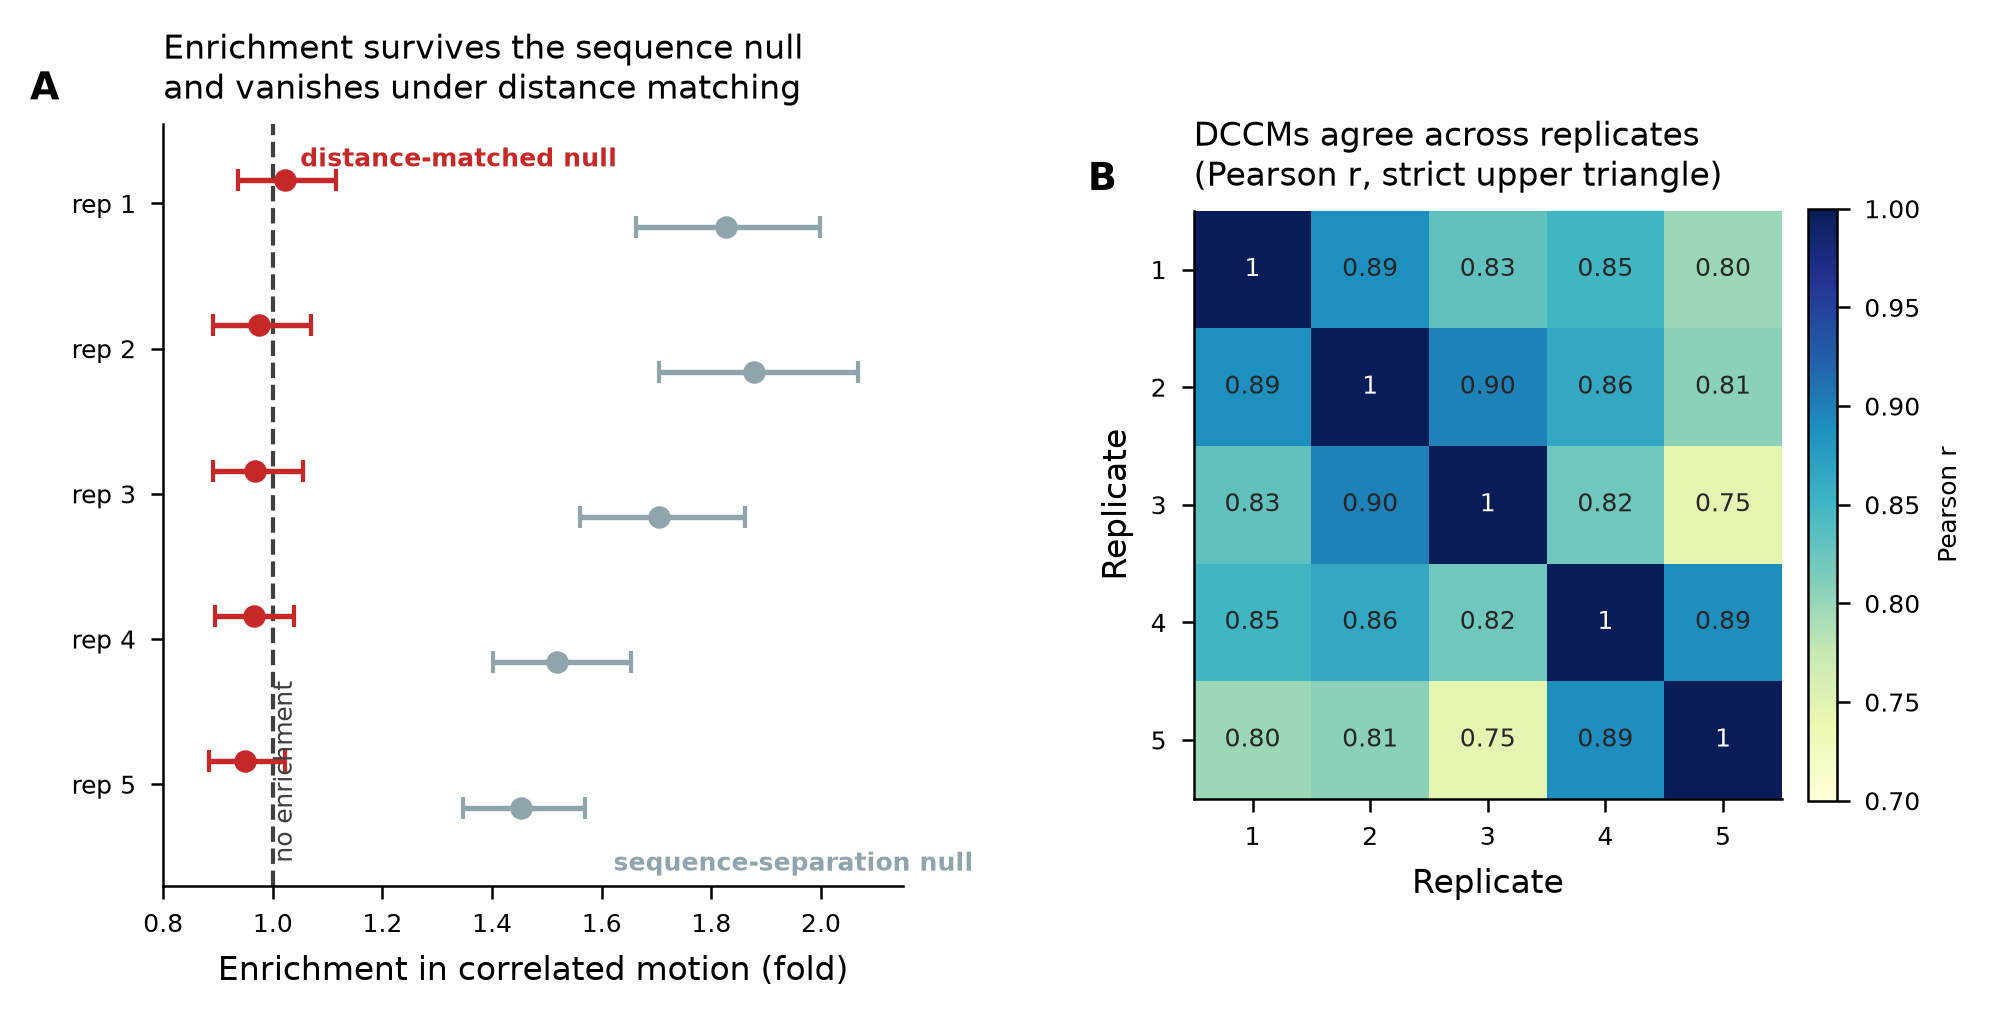
\includegraphics[width=15cm]{FIGURE_S1_replicates.png}
\end{center}
\caption{Reproducibility of the dynamic analysis across five independent 100 ns trajectories of the monomeric EGFR kinase domain (500 ns aggregate). \textbf{(A)} Enrichment in correlated motion of the 500 most strongly co-evolving distal pairs, computed separately for each replicate against a null matched on sequence separation ($|i-j|>5$) and against a null additionally matched on C\textalpha{}--C\textalpha{} distance in 2~\AA{} bins. Horizontal bars are bootstrap 95\% confidence intervals over 2{,}000 replicates; the dashed line marks the absence of enrichment. Replicate 1 is the published trajectory. Every replicate reproduces the enrichment under the sequence-separation null and its disappearance under distance matching. \textbf{(B)} Pearson correlation between replicate dynamic cross-correlation matrices, computed over the strict upper triangle of the $253\times253$ matrix spanning residues 714--966. Cell values are $r$; the colour scale begins at 0.70 rather than 0.}
\label{fig:replicates}
\end{figure}

\begin{table}[h!]
\caption{Replicate molecular dynamics: provenance and per-replicate statistics. Replicate 1 is the published run; replicates 2--5 were initialised with independent velocities from the same NPT configuration (identical \texttt{npt.gro}, \texttt{npt.cpt} and \texttt{topol.top} SHA256) through a 1~ns re-equilibration at 310~K, after which production parameters were identical to replicate 1 in every setting. Enrichment is the ratio of mean absolute dynamic correlation in the 500 most strongly co-evolving distal pairs to the matched null, with bootstrap 95\% confidence intervals in brackets. Throughput is the GROMACS \texttt{Performance} value from each production log.}
\label{tab:replicates}
\footnotesize
\begin{center}
\begin{tabular}{llllll}
\hline
Replicate & Seed & GROMACS build & ns/day & $r$ vs rep 1 & Enrichment [95\% CI] \\
 & & & & & sequence null \quad distance-matched \\
\hline
  1 & n/a (published run) & 2025.2 site module & 418 & -- & 1.83 [1.66, 2.00] & 1.02 [0.94, 1.12] \\
  2 & 20250002 & 2025.2 conda-forge (AVX2\_256) & 411 & 0.888 & 1.88 [1.70, 2.07] & 0.98 [0.89, 1.07] \\
  3 & 20250003 & 2025.2 conda-forge (AVX2\_256) & 400 & 0.830 & 1.71 [1.56, 1.86] & 0.97 [0.89, 1.06] \\
  4 & 20250004 & 2025.2 conda-forge (AVX2\_256) & 411 & 0.849 & 1.52 [1.40, 1.65] & 0.96 [0.89, 1.04] \\
  5 & 20250005 & 2025.2 conda-forge (AVX2\_256) & 418 & 0.798 & 1.45 [1.35, 1.57] & 0.95 [0.88, 1.02] \\
\hline
\end{tabular}
\end{center}
\end{table}

\end{document}
